\documentclass[twoside]{book}

% Packages required by doxygen
\usepackage{fixltx2e}
\usepackage{calc}
\usepackage{doxygen}
\usepackage[export]{adjustbox} % also loads graphicx
\usepackage{graphicx}
\usepackage[utf8]{inputenc}
\usepackage{makeidx}
\usepackage{multicol}
\usepackage{multirow}
\PassOptionsToPackage{warn}{textcomp}
\usepackage{textcomp}
\usepackage[nointegrals]{wasysym}
\usepackage[table]{xcolor}

% Font selection
\usepackage[T1]{fontenc}
\usepackage[scaled=.90]{helvet}
\usepackage{courier}
\usepackage{amssymb}
\usepackage{sectsty}
\renewcommand{\familydefault}{\sfdefault}
\allsectionsfont{%
  \fontseries{bc}\selectfont%
  \color{darkgray}%
}
\renewcommand{\DoxyLabelFont}{%
  \fontseries{bc}\selectfont%
  \color{darkgray}%
}
\newcommand{\+}{\discretionary{\mbox{\scriptsize$\hookleftarrow$}}{}{}}

% Page & text layout
\usepackage{geometry}
\geometry{%
  a4paper,%
  top=2.5cm,%
  bottom=2.5cm,%
  left=2.5cm,%
  right=2.5cm%
}
\tolerance=750
\hfuzz=15pt
\hbadness=750
\setlength{\emergencystretch}{15pt}
\setlength{\parindent}{0cm}
\setlength{\parskip}{3ex plus 2ex minus 2ex}
\makeatletter
\renewcommand{\paragraph}{%
  \@startsection{paragraph}{4}{0ex}{-1.0ex}{1.0ex}{%
    \normalfont\normalsize\bfseries\SS@parafont%
  }%
}
\renewcommand{\subparagraph}{%
  \@startsection{subparagraph}{5}{0ex}{-1.0ex}{1.0ex}{%
    \normalfont\normalsize\bfseries\SS@subparafont%
  }%
}
\makeatother

% Headers & footers
\usepackage{fancyhdr}
\pagestyle{fancyplain}
\fancyhead[LE]{\fancyplain{}{\bfseries\thepage}}
\fancyhead[CE]{\fancyplain{}{}}
\fancyhead[RE]{\fancyplain{}{\bfseries\leftmark}}
\fancyhead[LO]{\fancyplain{}{\bfseries\rightmark}}
\fancyhead[CO]{\fancyplain{}{}}
\fancyhead[RO]{\fancyplain{}{\bfseries\thepage}}
\fancyfoot[LE]{\fancyplain{}{}}
\fancyfoot[CE]{\fancyplain{}{}}
\fancyfoot[RE]{\fancyplain{}{\bfseries\scriptsize Generated by Doxygen }}
\fancyfoot[LO]{\fancyplain{}{\bfseries\scriptsize Generated by Doxygen }}
\fancyfoot[CO]{\fancyplain{}{}}
\fancyfoot[RO]{\fancyplain{}{}}
\renewcommand{\footrulewidth}{0.4pt}
\renewcommand{\chaptermark}[1]{%
  \markboth{#1}{}%
}
\renewcommand{\sectionmark}[1]{%
  \markright{\thesection\ #1}%
}

% Indices & bibliography
\usepackage{natbib}
\usepackage[titles]{tocloft}
\setcounter{tocdepth}{3}
\setcounter{secnumdepth}{5}
\makeindex

% Hyperlinks (required, but should be loaded last)
\usepackage{ifpdf}
\ifpdf
  \usepackage[pdftex,pagebackref=true]{hyperref}
\else
  \usepackage[ps2pdf,pagebackref=true]{hyperref}
\fi
\hypersetup{%
  colorlinks=true,%
  linkcolor=blue,%
  citecolor=blue,%
  unicode%
}

% Custom commands
\newcommand{\clearemptydoublepage}{%
  \newpage{\pagestyle{empty}\cleardoublepage}%
}

\usepackage{caption}
\captionsetup{labelsep=space,justification=centering,font={bf},singlelinecheck=off,skip=4pt,position=top}

%===== C O N T E N T S =====

\begin{document}

% Titlepage & ToC
\hypersetup{pageanchor=false,
             bookmarksnumbered=true,
             pdfencoding=unicode
            }
\pagenumbering{roman}
\begin{titlepage}
\vspace*{7cm}
\begin{center}%
{\Large Multimodal Dataset Creation }\\
\vspace*{1cm}
{\large Generated by Doxygen 1.8.11}\\
\end{center}
\end{titlepage}
\clearemptydoublepage
\tableofcontents
\clearemptydoublepage
\pagenumbering{arabic}
\hypersetup{pageanchor=true}

%--- Begin generated contents ---
\chapter{Namespace Index}
\section{Namespace List}
Here is a list of all documented namespaces with brief descriptions\+:\begin{DoxyCompactList}
\item\contentsline{section}{\hyperlink{namespacefake__node__pc_1_1py}{fake\+\_\+node\+\_\+pc.\+py} \\*This node is created for the creation of fake rosmessage sensor\+\_\+msgs/\+Point\+Cloud2, setting all values for Kinect Node Taking into account the structure of this type of message (docs.\+ros.\+org/api/sensor\+\_\+msgs/html/msg/\+Point\+Cluoud2.html) }{\pageref{namespacefake__node__pc_1_1py}}{}
\item\contentsline{section}{\hyperlink{namespaceGUI__node_1_1py}{G\+U\+I\+\_\+node.\+py} \\*This module shows the interface of the architecture whith the configuration and the recording windows }{\pageref{namespaceGUI__node_1_1py}}{}
\item\contentsline{section}{\hyperlink{namespaceKinect__node_1_1py}{Kinect\+\_\+node.\+py} \\*This node is the node capable of taking specific data (sensor\+\_\+msgs/\+Point\+Cloud2) from \hyperlink{classKinect__node_1_1Kinect}{Kinect} (or from the fake\+\_\+node\+\_\+\+Pc) and publish a topic with these }{\pageref{namespaceKinect__node_1_1py}}{}
\item\contentsline{section}{\hyperlink{namespacemocap__fake_1_1cpp}{mocap\+\_\+fake\+::cpp} }{\pageref{namespacemocap__fake_1_1cpp}}{}
\item\contentsline{section}{\hyperlink{namespaceMocap__node_1_1py}{Mocap\+\_\+node.\+py} \\*This node is the node capable of taking specific data (std\+\_\+msgs.\+msg/\+Float32\+Multi\+Array) from \hyperlink{classMocap__node_1_1Mocap}{Mocap} and publish a topic with these }{\pageref{namespaceMocap__node_1_1py}}{}
\item\contentsline{section}{\hyperlink{namespaceRecorder__IMU_1_1py}{Recorder\+\_\+\+I\+M\+U.\+py} \\*This node is created for recording all data from Smartwatch in a Rosbag }{\pageref{namespaceRecorder__IMU_1_1py}}{}
\item\contentsline{section}{\hyperlink{namespaceRecorder__mocap_1_1py}{Recorder\+\_\+mocap.\+py} \\*This node is created for recording all datas from Mocap in a Rosbag }{\pageref{namespaceRecorder__mocap_1_1py}}{}
\item\contentsline{section}{\hyperlink{namespaceRecorder__PC_1_1py}{Recorder\+\_\+\+P\+C.\+py} \\*This node is created for recording all datas from Kinect in a Rosbag }{\pageref{namespaceRecorder__PC_1_1py}}{}
\item\contentsline{section}{\hyperlink{namespaceSmartwatch__node_1_1py}{Smartwatch\+\_\+node.\+py} \\*This node is the node capable of taking specific data (sensor\+\_\+msgs/\+Imu) from Smartwatch (or from the fake\+\_\+node\+\_\+\+Imu) and publish a topic with these }{\pageref{namespaceSmartwatch__node_1_1py}}{}
\end{DoxyCompactList}

\chapter{Hierarchical Index}
\section{Class Hierarchy}
This inheritance list is sorted roughly, but not completely, alphabetically\+:\begin{DoxyCompactList}
\item object\begin{DoxyCompactList}
\item \contentsline{section}{fake\+\_\+node\+\_\+imu.\+Fake\+Imu}{\pageref{classfake__node__imu_1_1FakeImu}}{}
\item \contentsline{section}{fake\+\_\+node\+\_\+pc.\+Custom\+Point\+Cloud}{\pageref{classfake__node__pc_1_1CustomPointCloud}}{}
\item \contentsline{section}{Kinect\+\_\+node.\+Kinect}{\pageref{classKinect__node_1_1Kinect}}{}
\item \contentsline{section}{Mocap\+\_\+node.\+Mocap}{\pageref{classMocap__node_1_1Mocap}}{}
\item \contentsline{section}{Recorder\+\_\+\+I\+M\+U.\+Recorder\+Imu}{\pageref{classRecorder__IMU_1_1RecorderImu}}{}
\item \contentsline{section}{Recorder\+\_\+mocap.\+Recorder\+Mocap}{\pageref{classRecorder__mocap_1_1RecorderMocap}}{}
\item \contentsline{section}{Recorder\+\_\+\+P\+C.\+Recorder\+PC}{\pageref{classRecorder__PC_1_1RecorderPC}}{}
\item \contentsline{section}{Smartwatch\+\_\+node.\+Fromsmart}{\pageref{classSmartwatch__node_1_1Fromsmart}}{}
\end{DoxyCompactList}
\item Q\+Main\+Window\begin{DoxyCompactList}
\item \contentsline{section}{G\+U\+I\+\_\+node.\+Main\+Window}{\pageref{classGUI__node_1_1MainWindow}}{}
\end{DoxyCompactList}
\end{DoxyCompactList}

\chapter{Class Index}
\section{Class List}
Here are the classes, structs, unions and interfaces with brief descriptions\+:\begin{DoxyCompactList}
\item\contentsline{section}{\hyperlink{classfake__node__pc_1_1CustomPointCloud}{fake\+\_\+node\+\_\+pc.\+Custom\+Point\+Cloud} \\*Class custom\+Point\+Cloud }{\pageref{classfake__node__pc_1_1CustomPointCloud}}{}
\item\contentsline{section}{\hyperlink{classfake__node__imu_1_1FakeImu}{fake\+\_\+node\+\_\+imu.\+Fake\+Imu} \\*Class \hyperlink{classfake__node__imu_1_1FakeImu}{Fake\+Imu} }{\pageref{classfake__node__imu_1_1FakeImu}}{}
\item\contentsline{section}{\hyperlink{classSmartwatch__node_1_1Fromsmart}{Smartwatch\+\_\+node.\+Fromsmart} \\*Class From\+Smart }{\pageref{classSmartwatch__node_1_1Fromsmart}}{}
\item\contentsline{section}{\hyperlink{classKinect__node_1_1Kinect}{Kinect\+\_\+node.\+Kinect} \\*Class \hyperlink{classKinect__node_1_1Kinect}{Kinect} }{\pageref{classKinect__node_1_1Kinect}}{}
\item\contentsline{section}{\hyperlink{classGUI__node_1_1MainWindow}{G\+U\+I\+\_\+node.\+Main\+Window} \\*Class \hyperlink{classGUI__node_1_1MainWindow}{Main\+Window} }{\pageref{classGUI__node_1_1MainWindow}}{}
\item\contentsline{section}{\hyperlink{classMocap__node_1_1Mocap}{Mocap\+\_\+node.\+Mocap} \\*Class \hyperlink{classMocap__node_1_1Mocap}{Mocap} }{\pageref{classMocap__node_1_1Mocap}}{}
\item\contentsline{section}{\hyperlink{classRecorder__IMU_1_1RecorderImu}{Recorder\+\_\+\+I\+M\+U.\+Recorder\+Imu} \\*Class \hyperlink{classRecorder__IMU_1_1RecorderImu}{Recorder\+Imu} }{\pageref{classRecorder__IMU_1_1RecorderImu}}{}
\item\contentsline{section}{\hyperlink{classRecorder__mocap_1_1RecorderMocap}{Recorder\+\_\+mocap.\+Recorder\+Mocap} \\*Class \hyperlink{classRecorder__mocap_1_1RecorderMocap}{Recorder\+Mocap} }{\pageref{classRecorder__mocap_1_1RecorderMocap}}{}
\item\contentsline{section}{\hyperlink{classRecorder__PC_1_1RecorderPC}{Recorder\+\_\+\+P\+C.\+Recorder\+PC} \\*Class \hyperlink{classRecorder__PC_1_1RecorderPC}{Recorder\+PC} }{\pageref{classRecorder__PC_1_1RecorderPC}}{}
\end{DoxyCompactList}

\chapter{Namespace Documentation}
\hypertarget{namespacefake__node__pc_1_1py}{}\section{fake\+\_\+node\+\_\+pc.\+py Namespace Reference}
\label{namespacefake__node__pc_1_1py}\index{fake\+\_\+node\+\_\+pc.\+py@{fake\+\_\+node\+\_\+pc.\+py}}


This node is created for the creation of fake rosmessage sensor\+\_\+msgs/\+Point\+Cloud2, setting all values for Kinect Node Taking into account the structure of this type of message (docs.\+ros.\+org/api/sensor\+\_\+msgs/html/msg/\+Point\+Cluoud2.html)  




\subsection{Detailed Description}
This node is created for the creation of fake rosmessage sensor\+\_\+msgs/\+Point\+Cloud2, setting all values for Kinect Node Taking into account the structure of this type of message (docs.\+ros.\+org/api/sensor\+\_\+msgs/html/msg/\+Point\+Cluoud2.html) 
\hypertarget{namespaceGUI__node_1_1py}{}\section{G\+U\+I\+\_\+node.\+py Namespace Reference}
\label{namespaceGUI__node_1_1py}\index{G\+U\+I\+\_\+node.\+py@{G\+U\+I\+\_\+node.\+py}}


This module shows the interface of the architecture whith the configuration and the recording windows.  




\subsection{Detailed Description}
This module shows the interface of the architecture whith the configuration and the recording windows. 
\hypertarget{namespaceKinect__node_1_1py}{}\section{Kinect\+\_\+node.\+py Namespace Reference}
\label{namespaceKinect__node_1_1py}\index{Kinect\+\_\+node.\+py@{Kinect\+\_\+node.\+py}}


This node is the node capable of taking specific data (sensor\+\_\+msgs/\+Point\+Cloud2) from \hyperlink{classKinect__node_1_1Kinect}{Kinect} (or from the fake\+\_\+node\+\_\+\+Pc) and publish a topic with these.  




\subsection{Detailed Description}
This node is the node capable of taking specific data (sensor\+\_\+msgs/\+Point\+Cloud2) from \hyperlink{classKinect__node_1_1Kinect}{Kinect} (or from the fake\+\_\+node\+\_\+\+Pc) and publish a topic with these. 


\hypertarget{namespacemocap__fake_1_1cpp}{}\section{mocap\+\_\+fake\+:\+:cpp Namespace Reference}
\label{namespacemocap__fake_1_1cpp}\index{mocap\+\_\+fake\+::cpp@{mocap\+\_\+fake\+::cpp}}


\subsection{Detailed Description}
This node computes fake mocap data 
\hypertarget{namespaceMocap__node_1_1py}{}\section{Mocap\+\_\+node.\+py Namespace Reference}
\label{namespaceMocap__node_1_1py}\index{Mocap\+\_\+node.\+py@{Mocap\+\_\+node.\+py}}


This node is the node capable of taking specific data (std\+\_\+msgs.\+msg/\+Float32\+Multi\+Array) from \hyperlink{classMocap__node_1_1Mocap}{Mocap} and publish a topic with these.  




\subsection{Detailed Description}
This node is the node capable of taking specific data (std\+\_\+msgs.\+msg/\+Float32\+Multi\+Array) from \hyperlink{classMocap__node_1_1Mocap}{Mocap} and publish a topic with these. 


\hypertarget{namespaceRecorder__IMU_1_1py}{}\section{Recorder\+\_\+\+I\+M\+U.\+py Namespace Reference}
\label{namespaceRecorder__IMU_1_1py}\index{Recorder\+\_\+\+I\+M\+U.\+py@{Recorder\+\_\+\+I\+M\+U.\+py}}


This node is created for recording all data from Smartwatch in a Rosbag.  




\subsection{Detailed Description}
This node is created for recording all data from Smartwatch in a Rosbag. 


\hypertarget{namespaceRecorder__mocap_1_1py}{}\section{Recorder\+\_\+mocap.\+py Namespace Reference}
\label{namespaceRecorder__mocap_1_1py}\index{Recorder\+\_\+mocap.\+py@{Recorder\+\_\+mocap.\+py}}


This node is created for recording all datas from Mocap in a Rosbag.  




\subsection{Detailed Description}
This node is created for recording all datas from Mocap in a Rosbag. 


\hypertarget{namespaceRecorder__PC_1_1py}{}\section{Recorder\+\_\+\+P\+C.\+py Namespace Reference}
\label{namespaceRecorder__PC_1_1py}\index{Recorder\+\_\+\+P\+C.\+py@{Recorder\+\_\+\+P\+C.\+py}}


This node is created for recording all datas from Kinect in a Rosbag.  




\subsection{Detailed Description}
This node is created for recording all datas from Kinect in a Rosbag. 


\hypertarget{namespaceSmartwatch__node_1_1py}{}\section{Smartwatch\+\_\+node.\+py Namespace Reference}
\label{namespaceSmartwatch__node_1_1py}\index{Smartwatch\+\_\+node.\+py@{Smartwatch\+\_\+node.\+py}}


This node is the node capable of taking specific data (sensor\+\_\+msgs/\+Imu) from Smartwatch (or from the fake\+\_\+node\+\_\+\+Imu) and publish a topic with these.  




\subsection{Detailed Description}
This node is the node capable of taking specific data (sensor\+\_\+msgs/\+Imu) from Smartwatch (or from the fake\+\_\+node\+\_\+\+Imu) and publish a topic with these. 


\chapter{Class Documentation}
\hypertarget{classfake__node__pc_1_1CustomPointCloud}{}\section{fake\+\_\+node\+\_\+pc.\+Custom\+Point\+Cloud Class Reference}
\label{classfake__node__pc_1_1CustomPointCloud}\index{fake\+\_\+node\+\_\+pc.\+Custom\+Point\+Cloud@{fake\+\_\+node\+\_\+pc.\+Custom\+Point\+Cloud}}


class custom\+Point\+Cloud  




Inheritance diagram for fake\+\_\+node\+\_\+pc.\+Custom\+Point\+Cloud\+:
\nopagebreak
\begin{figure}[H]
\begin{center}
\leavevmode
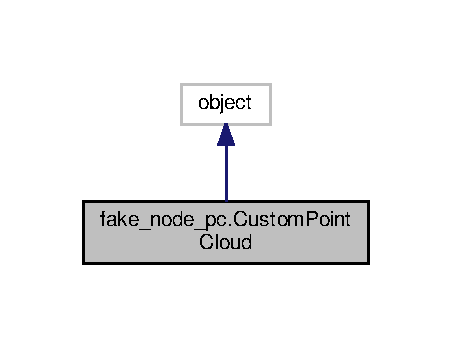
\includegraphics[width=217pt]{classfake__node__pc_1_1CustomPointCloud__inherit__graph}
\end{center}
\end{figure}


Collaboration diagram for fake\+\_\+node\+\_\+pc.\+Custom\+Point\+Cloud\+:
\nopagebreak
\begin{figure}[H]
\begin{center}
\leavevmode
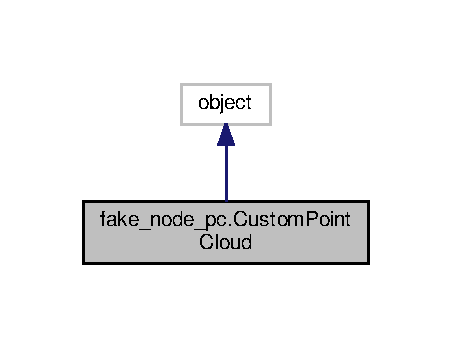
\includegraphics[width=217pt]{classfake__node__pc_1_1CustomPointCloud__coll__graph}
\end{center}
\end{figure}
\subsection*{Public Member Functions}
\begin{DoxyCompactItemize}
\item 
def {\bfseries \+\_\+\+\_\+init\+\_\+\+\_\+} (self)\hypertarget{classfake__node__pc_1_1CustomPointCloud_a9a10f269e06529110e89a3a5955cf133}{}\label{classfake__node__pc_1_1CustomPointCloud_a9a10f269e06529110e89a3a5955cf133}

\end{DoxyCompactItemize}
\subsection*{Public Attributes}
\begin{DoxyCompactItemize}
\item 
{\bfseries publisher}\hypertarget{classfake__node__pc_1_1CustomPointCloud_a8ad08026b7831dfdf3a0088c6c6a5c05}{}\label{classfake__node__pc_1_1CustomPointCloud_a8ad08026b7831dfdf3a0088c6c6a5c05}

\end{DoxyCompactItemize}


\subsection{Detailed Description}
class custom\+Point\+Cloud 

The documentation for this class was generated from the following file\+:\begin{DoxyCompactItemize}
\item 
fake\+\_\+node\+\_\+pc.\+py\end{DoxyCompactItemize}

\hypertarget{classfake__node__imu_1_1FakeImu}{}\section{fake\+\_\+node\+\_\+imu.\+Fake\+Imu Class Reference}
\label{classfake__node__imu_1_1FakeImu}\index{fake\+\_\+node\+\_\+imu.\+Fake\+Imu@{fake\+\_\+node\+\_\+imu.\+Fake\+Imu}}


class \hyperlink{classfake__node__imu_1_1FakeImu}{Fake\+Imu}  




Inheritance diagram for fake\+\_\+node\+\_\+imu.\+Fake\+Imu\+:
\nopagebreak
\begin{figure}[H]
\begin{center}
\leavevmode
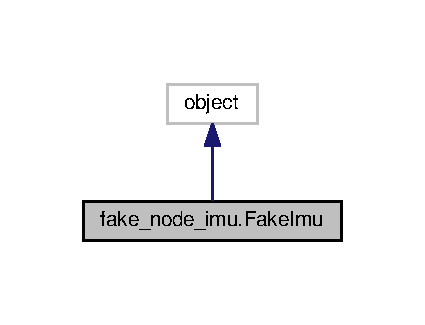
\includegraphics[width=204pt]{classfake__node__imu_1_1FakeImu__inherit__graph}
\end{center}
\end{figure}


Collaboration diagram for fake\+\_\+node\+\_\+imu.\+Fake\+Imu\+:
\nopagebreak
\begin{figure}[H]
\begin{center}
\leavevmode
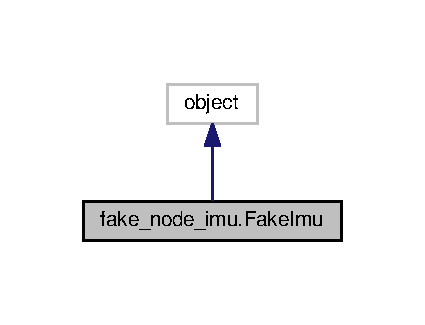
\includegraphics[width=204pt]{classfake__node__imu_1_1FakeImu__coll__graph}
\end{center}
\end{figure}
\subsection*{Public Member Functions}
\begin{DoxyCompactItemize}
\item 
def {\bfseries init} (self)\hypertarget{classfake__node__imu_1_1FakeImu_a672d5a8b50d8996b4e9ed1c57b0815c1}{}\label{classfake__node__imu_1_1FakeImu_a672d5a8b50d8996b4e9ed1c57b0815c1}

\item 
def \hyperlink{classfake__node__imu_1_1FakeImu_a52b19b270ea59d8df00fbad99d0b39f2}{run} (self)
\begin{DoxyCompactList}\small\item\em Fill in the sensor data setting to 0. \end{DoxyCompactList}\end{DoxyCompactItemize}
\subsection*{Public Attributes}
\begin{DoxyCompactItemize}
\item 
{\bfseries update\+\_\+rate}\hypertarget{classfake__node__imu_1_1FakeImu_afc4cf311196ce94a204ae76d67fec37f}{}\label{classfake__node__imu_1_1FakeImu_afc4cf311196ce94a204ae76d67fec37f}

\item 
{\bfseries pub\+\_\+imu}\hypertarget{classfake__node__imu_1_1FakeImu_a0e738903cc497b62692d80dc19179efb}{}\label{classfake__node__imu_1_1FakeImu_a0e738903cc497b62692d80dc19179efb}

\end{DoxyCompactItemize}
\subsection*{Static Public Attributes}
\begin{DoxyCompactItemize}
\item 
\hyperlink{classfake__node__imu_1_1FakeImu_a3de5593ad57683acd9a7878edd709ecc}{fake\+\_\+imu}\hypertarget{classfake__node__imu_1_1FakeImu_a3de5593ad57683acd9a7878edd709ecc}{}\label{classfake__node__imu_1_1FakeImu_a3de5593ad57683acd9a7878edd709ecc}

\begin{DoxyCompactList}\small\item\em Create a new Fakedata\+Imu object and fill in in its contents. \end{DoxyCompactList}\item 
\hyperlink{classfake__node__imu_1_1FakeImu_aa5cadb2f5d0a38d7cb5add38dd7d1051}{stamp}\hypertarget{classfake__node__imu_1_1FakeImu_aa5cadb2f5d0a38d7cb5add38dd7d1051}{}\label{classfake__node__imu_1_1FakeImu_aa5cadb2f5d0a38d7cb5add38dd7d1051}

\begin{DoxyCompactList}\small\item\em Fill in the header information. \end{DoxyCompactList}\item 
{\bfseries frame\+\_\+id}\hypertarget{classfake__node__imu_1_1FakeImu_aa42cc05ac350d8ddd4e4272b70ea89eb}{}\label{classfake__node__imu_1_1FakeImu_aa42cc05ac350d8ddd4e4272b70ea89eb}

\end{DoxyCompactItemize}


\subsection{Detailed Description}
class \hyperlink{classfake__node__imu_1_1FakeImu}{Fake\+Imu} 

\subsection{Member Function Documentation}
\index{fake\+\_\+node\+\_\+imu\+::\+Fake\+Imu@{fake\+\_\+node\+\_\+imu\+::\+Fake\+Imu}!run@{run}}
\index{run@{run}!fake\+\_\+node\+\_\+imu\+::\+Fake\+Imu@{fake\+\_\+node\+\_\+imu\+::\+Fake\+Imu}}
\subsubsection[{\texorpdfstring{run(self)}{run(self)}}]{\setlength{\rightskip}{0pt plus 5cm}def fake\+\_\+node\+\_\+imu.\+Fake\+Imu.\+run (
\begin{DoxyParamCaption}
\item[{}]{self}
\end{DoxyParamCaption}
)}\hypertarget{classfake__node__imu_1_1FakeImu_a52b19b270ea59d8df00fbad99d0b39f2}{}\label{classfake__node__imu_1_1FakeImu_a52b19b270ea59d8df00fbad99d0b39f2}


Fill in the sensor data setting to 0. 

function to publish data into a topic 

The documentation for this class was generated from the following file\+:\begin{DoxyCompactItemize}
\item 
fake\+\_\+node\+\_\+imu.\+py\end{DoxyCompactItemize}

\hypertarget{classSmartwatch__node_1_1Fromsmart}{}\section{Smartwatch\+\_\+node.\+Fromsmart Class Reference}
\label{classSmartwatch__node_1_1Fromsmart}\index{Smartwatch\+\_\+node.\+Fromsmart@{Smartwatch\+\_\+node.\+Fromsmart}}


class From\+Smart  




Inheritance diagram for Smartwatch\+\_\+node.\+Fromsmart\+:
\nopagebreak
\begin{figure}[H]
\begin{center}
\leavevmode
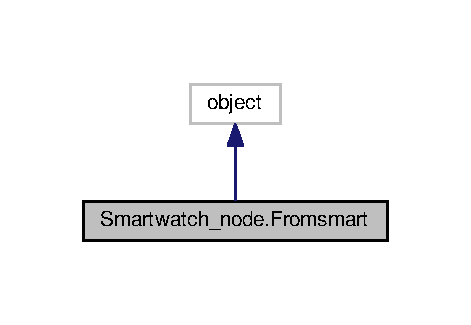
\includegraphics[width=226pt]{classSmartwatch__node_1_1Fromsmart__inherit__graph}
\end{center}
\end{figure}


Collaboration diagram for Smartwatch\+\_\+node.\+Fromsmart\+:
\nopagebreak
\begin{figure}[H]
\begin{center}
\leavevmode
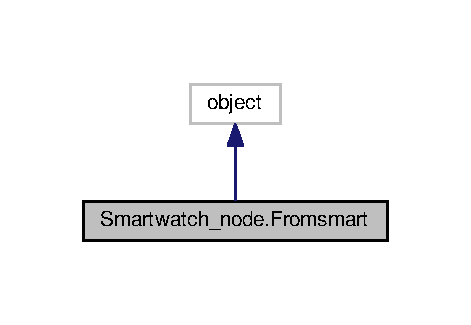
\includegraphics[width=226pt]{classSmartwatch__node_1_1Fromsmart__coll__graph}
\end{center}
\end{figure}
\subsection*{Public Member Functions}
\begin{DoxyCompactItemize}
\item 
def {\bfseries init} (self)\hypertarget{classSmartwatch__node_1_1Fromsmart_a4f503d9ce16992632a0c672dc718cb0b}{}\label{classSmartwatch__node_1_1Fromsmart_a4f503d9ce16992632a0c672dc718cb0b}

\end{DoxyCompactItemize}
\subsection*{Public Attributes}
\begin{DoxyCompactItemize}
\item 
{\bfseries data1}\hypertarget{classSmartwatch__node_1_1Fromsmart_a9191ed73fe4af664c880c76b79ec68b9}{}\label{classSmartwatch__node_1_1Fromsmart_a9191ed73fe4af664c880c76b79ec68b9}

\item 
{\bfseries flagstart}\hypertarget{classSmartwatch__node_1_1Fromsmart_a7940f096e122a79720da8b314a74e988}{}\label{classSmartwatch__node_1_1Fromsmart_a7940f096e122a79720da8b314a74e988}

\item 
\hyperlink{classSmartwatch__node_1_1Fromsmart_a6ee3e1ebd679e70496307898c2dbd390}{update\+\_\+rate}\hypertarget{classSmartwatch__node_1_1Fromsmart_a6ee3e1ebd679e70496307898c2dbd390}{}\label{classSmartwatch__node_1_1Fromsmart_a6ee3e1ebd679e70496307898c2dbd390}

\begin{DoxyCompactList}\small\item\em defining frequency \end{DoxyCompactList}\item 
{\bfseries data}\hypertarget{classSmartwatch__node_1_1Fromsmart_aa02d6526bb377e593efbe3a64ac00ffa}{}\label{classSmartwatch__node_1_1Fromsmart_aa02d6526bb377e593efbe3a64ac00ffa}

\item 
{\bfseries data\+Published}\hypertarget{classSmartwatch__node_1_1Fromsmart_a03c7946d143ce60db1e3fad5fc1637d6}{}\label{classSmartwatch__node_1_1Fromsmart_a03c7946d143ce60db1e3fad5fc1637d6}

\item 
\hyperlink{classSmartwatch__node_1_1Fromsmart_a15e21f550231b29281c85ee49fc6119f}{pub\+\_\+imu}\hypertarget{classSmartwatch__node_1_1Fromsmart_a15e21f550231b29281c85ee49fc6119f}{}\label{classSmartwatch__node_1_1Fromsmart_a15e21f550231b29281c85ee49fc6119f}

\begin{DoxyCompactList}\small\item\em creation of the topic with the intersting data \end{DoxyCompactList}\end{DoxyCompactItemize}


\subsection{Detailed Description}
class From\+Smart 

The documentation for this class was generated from the following file\+:\begin{DoxyCompactItemize}
\item 
Smartwatch\+\_\+node.\+py\end{DoxyCompactItemize}

\hypertarget{classKinect__node_1_1Kinect}{}\section{Kinect\+\_\+node.\+Kinect Class Reference}
\label{classKinect__node_1_1Kinect}\index{Kinect\+\_\+node.\+Kinect@{Kinect\+\_\+node.\+Kinect}}


class \hyperlink{classKinect__node_1_1Kinect}{Kinect}  




Inheritance diagram for Kinect\+\_\+node.\+Kinect\+:
\nopagebreak
\begin{figure}[H]
\begin{center}
\leavevmode
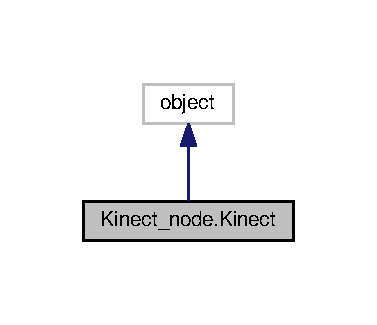
\includegraphics[width=181pt]{classKinect__node_1_1Kinect__inherit__graph}
\end{center}
\end{figure}


Collaboration diagram for Kinect\+\_\+node.\+Kinect\+:
\nopagebreak
\begin{figure}[H]
\begin{center}
\leavevmode
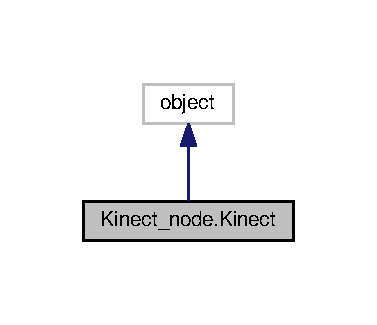
\includegraphics[width=181pt]{classKinect__node_1_1Kinect__coll__graph}
\end{center}
\end{figure}
\subsection*{Public Member Functions}
\begin{DoxyCompactItemize}
\item 
def {\bfseries init} (self)\hypertarget{classKinect__node_1_1Kinect_a89f83988b18b58069ad77bb441616524}{}\label{classKinect__node_1_1Kinect_a89f83988b18b58069ad77bb441616524}

\end{DoxyCompactItemize}
\subsection*{Public Attributes}
\begin{DoxyCompactItemize}
\item 
{\bfseries data1}\hypertarget{classKinect__node_1_1Kinect_a5f313fce01efc2bb22659e8ac579f6f8}{}\label{classKinect__node_1_1Kinect_a5f313fce01efc2bb22659e8ac579f6f8}

\item 
{\bfseries flag}\hypertarget{classKinect__node_1_1Kinect_a08b726f7c6d6fefbe15ed98325ce3a2a}{}\label{classKinect__node_1_1Kinect_a08b726f7c6d6fefbe15ed98325ce3a2a}

\item 
{\bfseries flagstart}\hypertarget{classKinect__node_1_1Kinect_a0fe62627028382ffa28b4354aa1cfea7}{}\label{classKinect__node_1_1Kinect_a0fe62627028382ffa28b4354aa1cfea7}

\item 
\hyperlink{classKinect__node_1_1Kinect_a08528ddb2bc98e179b6428ee1ce79e6e}{update\+\_\+rate}\hypertarget{classKinect__node_1_1Kinect_a08528ddb2bc98e179b6428ee1ce79e6e}{}\label{classKinect__node_1_1Kinect_a08528ddb2bc98e179b6428ee1ce79e6e}

\begin{DoxyCompactList}\small\item\em defining frequency \end{DoxyCompactList}\item 
{\bfseries data}\hypertarget{classKinect__node_1_1Kinect_a20848834d4823200459263f0486693df}{}\label{classKinect__node_1_1Kinect_a20848834d4823200459263f0486693df}

\item 
\hyperlink{classKinect__node_1_1Kinect_a97e982cd145341ebf4fadd5959bfb237}{pub}\hypertarget{classKinect__node_1_1Kinect_a97e982cd145341ebf4fadd5959bfb237}{}\label{classKinect__node_1_1Kinect_a97e982cd145341ebf4fadd5959bfb237}

\begin{DoxyCompactList}\small\item\em creation of a topic the interested data \end{DoxyCompactList}\end{DoxyCompactItemize}


\subsection{Detailed Description}
class \hyperlink{classKinect__node_1_1Kinect}{Kinect} 

The documentation for this class was generated from the following file\+:\begin{DoxyCompactItemize}
\item 
Kinect\+\_\+node.\+py\end{DoxyCompactItemize}

\hypertarget{classGUI__node_1_1MainWindow}{}\section{G\+U\+I\+\_\+node.\+Main\+Window Class Reference}
\label{classGUI__node_1_1MainWindow}\index{G\+U\+I\+\_\+node.\+Main\+Window@{G\+U\+I\+\_\+node.\+Main\+Window}}


class \hyperlink{classGUI__node_1_1MainWindow}{Main\+Window}  




Inheritance diagram for G\+U\+I\+\_\+node.\+Main\+Window\+:
\nopagebreak
\begin{figure}[H]
\begin{center}
\leavevmode
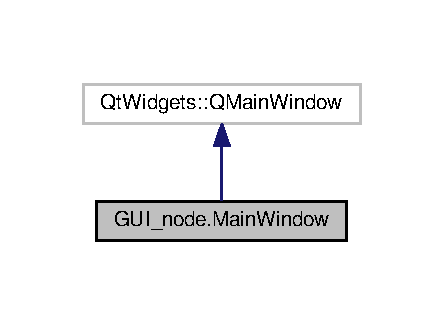
\includegraphics[width=213pt]{classGUI__node_1_1MainWindow__inherit__graph}
\end{center}
\end{figure}


Collaboration diagram for G\+U\+I\+\_\+node.\+Main\+Window\+:
\nopagebreak
\begin{figure}[H]
\begin{center}
\leavevmode
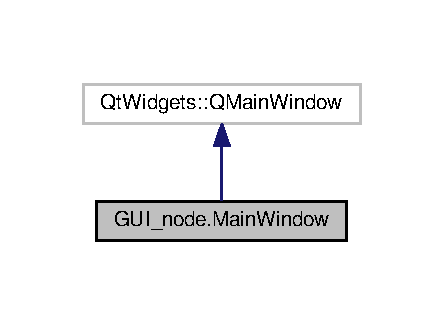
\includegraphics[width=213pt]{classGUI__node_1_1MainWindow__coll__graph}
\end{center}
\end{figure}
\subsection*{Public Member Functions}
\begin{DoxyCompactItemize}
\item 
def {\bfseries \+\_\+\+\_\+init\+\_\+\+\_\+} (self, parent=None)\hypertarget{classGUI__node_1_1MainWindow_a91cc7c05ff8bf1511cd5261e7325a126}{}\label{classGUI__node_1_1MainWindow_a91cc7c05ff8bf1511cd5261e7325a126}

\item 
def \hyperlink{classGUI__node_1_1MainWindow_a9d070f64208c98d3567b1275b7d35e07}{start\+Welcome\+Window} (self)
\begin{DoxyCompactList}\small\item\em function start\+Welcome\+Window Function that shows the welcome window \end{DoxyCompactList}\item 
def \hyperlink{classGUI__node_1_1MainWindow_add9380f974135deaf470c8ed010d8726}{start\+Configuration\+Tutorial\+Window} (self)
\begin{DoxyCompactList}\small\item\em function start\+Configuration\+Tutorial\+Window Function that shows the configuration tutorial window \end{DoxyCompactList}\item 
def \hyperlink{classGUI__node_1_1MainWindow_a835e01e508e046a1f89c6422704dc9be}{configuration\+Tutorial\+Second\+Part} (self)
\begin{DoxyCompactList}\small\item\em function configuration\+Tutorial\+Second\+Part Function that shows the second part of the configuration tutorial \end{DoxyCompactList}\item 
def \hyperlink{classGUI__node_1_1MainWindow_a095f642c8d8aba490bbae131c8b6c89b}{configuration\+Tutorial\+Third\+Part} (self)
\begin{DoxyCompactList}\small\item\em function configuration\+Tutorial\+Third\+Part Function that shows the third part of the configuration tutorial \end{DoxyCompactList}\item 
def \hyperlink{classGUI__node_1_1MainWindow_abe0d2c5692579f0e853c22cd9d9885d5}{start\+Recording\+Tutorial\+Window} (self)
\begin{DoxyCompactList}\small\item\em function start\+Recording\+Tutorial\+Window Function that shows the recording tutorial window \end{DoxyCompactList}\item 
def \hyperlink{classGUI__node_1_1MainWindow_a33c8780a5d36c6cc297cf02eb9f5adbf}{start\+Configuration\+Window} (self)
\begin{DoxyCompactList}\small\item\em function start\+Configuration\+Window Function that shows the configuration window \end{DoxyCompactList}\item 
def \hyperlink{classGUI__node_1_1MainWindow_a82192239f14fe38d98ad04569e640f4e}{select\+Casual\+Sequence} (self)
\begin{DoxyCompactList}\small\item\em function select\+Casual\+Sequence Management of the mutual exclusion between choosing a random sequence or a predefined one \end{DoxyCompactList}\item 
def \hyperlink{classGUI__node_1_1MainWindow_a4b7adbe5d7b9fb86d0a303a9ca6b9877}{go\+To\+Recording} (self)
\begin{DoxyCompactList}\small\item\em function go\+To\+Recording Function that shows the recording window \end{DoxyCompactList}\item 
def \hyperlink{classGUI__node_1_1MainWindow_aaa95191d6789b9f88ce6b44ca163292f}{save\+Personal\+Info} (self)
\begin{DoxyCompactList}\small\item\em function save\+Personal\+Info Function that save the personal informations temporarily before saving them into a file \end{DoxyCompactList}\item 
def \hyperlink{classGUI__node_1_1MainWindow_a7115adbcfd42afe1aa7cb18580b1dda7}{ask\+Gesture\+Sequence} (self)
\begin{DoxyCompactList}\small\item\em ask\+Gesture\+Sequence method Makes a request to the service to get the random gesture sequence \end{DoxyCompactList}\item 
def \hyperlink{classGUI__node_1_1MainWindow_a75c3a59f43f7efba27ee5c01c336143d}{recording\+Init} (self)
\begin{DoxyCompactList}\small\item\em function recording\+Init Function called when the Play button is clicked to start the countdown before the recording starts \end{DoxyCompactList}\item 
def \hyperlink{classGUI__node_1_1MainWindow_a67334f3548f8ff20e391d5d4840e4794}{show\+Countdown} (self)
\begin{DoxyCompactList}\small\item\em function show\+Countdown Function that shows the countdown on the recording window \end{DoxyCompactList}\item 
def \hyperlink{classGUI__node_1_1MainWindow_af3f78981958f0ec8a6b073f64a6a08c2}{sensors\+Init} (self)
\begin{DoxyCompactList}\small\item\em function sensors\+Init Function that publishes the correct start commands \end{DoxyCompactList}\item 
def \hyperlink{classGUI__node_1_1MainWindow_a3e94c0d07b7df8ac9e665ef001c5bd31}{create\+Recording\+Folder} (self)
\begin{DoxyCompactList}\small\item\em function create\+Recording\+Folder Function that creates the current recording folder \end{DoxyCompactList}\item 
def \hyperlink{classGUI__node_1_1MainWindow_acddcf8f2932ff86fc1ad189cf60ab720}{stop\+Recording} (self)
\begin{DoxyCompactList}\small\item\em function stop\+Recording Function that is called when the user presses the Stop button to halt the recording before the predefined time \end{DoxyCompactList}\item 
def \hyperlink{classGUI__node_1_1MainWindow_a1877e3df74eea96aba726dbe547987c8}{feedback\+Init} (self)
\begin{DoxyCompactList}\small\item\em function feedback\+Init Function that initializes the parameters needed for the feedback \end{DoxyCompactList}\item 
def \hyperlink{classGUI__node_1_1MainWindow_aadfd391d5efa53cbd6eee41968972bfe}{recording\+Feedback} (self)
\begin{DoxyCompactList}\small\item\em function recording\+Feedback Function that deals with updating the current time and eventually calling the update\+Image function \end{DoxyCompactList}\item 
def \hyperlink{classGUI__node_1_1MainWindow_ab6b0d212b93f190da018162d8374aa80}{update\+Image} (self, gesture\+Position)
\begin{DoxyCompactList}\small\item\em function update\+Image Function that updates the image to be shown to the user \end{DoxyCompactList}\end{DoxyCompactItemize}
\subsection*{Public Attributes}
\begin{DoxyCompactItemize}
\item 
\hyperlink{classGUI__node_1_1MainWindow_ab26e179eff19c4b964aa6bd36c91d595}{kinect\+Publisher}\hypertarget{classGUI__node_1_1MainWindow_ab26e179eff19c4b964aa6bd36c91d595}{}\label{classGUI__node_1_1MainWindow_ab26e179eff19c4b964aa6bd36c91d595}

\begin{DoxyCompactList}\small\item\em Create three topics in order to communicate the start/stop command to the sensors. \end{DoxyCompactList}\item 
{\bfseries smartwatch\+Publisher}\hypertarget{classGUI__node_1_1MainWindow_ac7aedba16d83e28a2952abc28968885e}{}\label{classGUI__node_1_1MainWindow_ac7aedba16d83e28a2952abc28968885e}

\item 
{\bfseries mocap\+Publisher}\hypertarget{classGUI__node_1_1MainWindow_ab359c61dae9dae4a812103ecf23d0e2c}{}\label{classGUI__node_1_1MainWindow_ab359c61dae9dae4a812103ecf23d0e2c}

\item 
\hyperlink{classGUI__node_1_1MainWindow_a02198b72f9182a5c79ee3834edf95108}{total\+Time}
\begin{DoxyCompactList}\small\item\em Variable to store the total recording time in seconds. \end{DoxyCompactList}\item 
\hyperlink{classGUI__node_1_1MainWindow_ad8b02713e5b5516ef657c7097cf54ca4}{recording\+Directory}\hypertarget{classGUI__node_1_1MainWindow_ad8b02713e5b5516ef657c7097cf54ca4}{}\label{classGUI__node_1_1MainWindow_ad8b02713e5b5516ef657c7097cf54ca4}

\begin{DoxyCompactList}\small\item\em Directory where all the current recording related files will be saved. \end{DoxyCompactList}\item 
\hyperlink{classGUI__node_1_1MainWindow_a45f694f080c9291370d9d58a5192c158}{working\+Directory}\hypertarget{classGUI__node_1_1MainWindow_a45f694f080c9291370d9d58a5192c158}{}\label{classGUI__node_1_1MainWindow_a45f694f080c9291370d9d58a5192c158}

\begin{DoxyCompactList}\small\item\em Retrieve the main folder. \end{DoxyCompactList}\item 
{\bfseries parent\+Directory}\hypertarget{classGUI__node_1_1MainWindow_a9eb8e938708adaffeb60bb74c39bd71c}{}\label{classGUI__node_1_1MainWindow_a9eb8e938708adaffeb60bb74c39bd71c}

\item 
\hyperlink{classGUI__node_1_1MainWindow_ad50097b037ad87eeef2243f2ec4194dd}{complete\+Gesture\+Sequence}
\begin{DoxyCompactList}\small\item\em List to store the gesture sequence to be performed. \end{DoxyCompactList}\item 
{\bfseries welcome\+\_\+\+Window}\hypertarget{classGUI__node_1_1MainWindow_a75ba2a822d88adf61f3d2e29480b54ed}{}\label{classGUI__node_1_1MainWindow_a75ba2a822d88adf61f3d2e29480b54ed}

\item 
{\bfseries welcome\+\_\+\+Widget}\hypertarget{classGUI__node_1_1MainWindow_a8403ef9c59e8b4b64797cb7628a3e4cd}{}\label{classGUI__node_1_1MainWindow_a8403ef9c59e8b4b64797cb7628a3e4cd}

\item 
{\bfseries configuration\+Tutorial\+\_\+\+Window}\hypertarget{classGUI__node_1_1MainWindow_a5ff5e55c9ced8975fa58ee08ccbdcec8}{}\label{classGUI__node_1_1MainWindow_a5ff5e55c9ced8975fa58ee08ccbdcec8}

\item 
{\bfseries configuration\+Tutorial\+\_\+\+Widget}\hypertarget{classGUI__node_1_1MainWindow_af81587b11d89cbca1b00aecf059d8ee7}{}\label{classGUI__node_1_1MainWindow_af81587b11d89cbca1b00aecf059d8ee7}

\item 
\hyperlink{classGUI__node_1_1MainWindow_a79061358e7ad20c614b2a60c12ef7691}{first\+Tutorial\+Directory}\hypertarget{classGUI__node_1_1MainWindow_a79061358e7ad20c614b2a60c12ef7691}{}\label{classGUI__node_1_1MainWindow_a79061358e7ad20c614b2a60c12ef7691}

\begin{DoxyCompactList}\small\item\em Show the first tutorial image. \end{DoxyCompactList}\item 
\hyperlink{classGUI__node_1_1MainWindow_a4e01d22041049f7266e34d9a59f8cb37}{second\+Tutorial\+Directory}
\begin{DoxyCompactList}\small\item\em Change the informative text. \end{DoxyCompactList}\item 
\hyperlink{classGUI__node_1_1MainWindow_a20e2d3b578d229d24d744e2d50269298}{third\+Tutorial\+Directory}
\begin{DoxyCompactList}\small\item\em Change the informative text. \end{DoxyCompactList}\item 
{\bfseries recording\+Tutorial\+\_\+\+Window}\hypertarget{classGUI__node_1_1MainWindow_aad2e758ee5e063c2ad4ef19f844c57dc}{}\label{classGUI__node_1_1MainWindow_aad2e758ee5e063c2ad4ef19f844c57dc}

\item 
{\bfseries recording\+Tutorial\+\_\+\+Widget}\hypertarget{classGUI__node_1_1MainWindow_a5c16c61707312e5a130e3ea3820e265b}{}\label{classGUI__node_1_1MainWindow_a5c16c61707312e5a130e3ea3820e265b}

\item 
{\bfseries configuration\+\_\+\+Window}\hypertarget{classGUI__node_1_1MainWindow_a4de2781d66d80d6b2952b23f4d560466}{}\label{classGUI__node_1_1MainWindow_a4de2781d66d80d6b2952b23f4d560466}

\item 
{\bfseries configuration\+\_\+\+Widget}\hypertarget{classGUI__node_1_1MainWindow_ab29ad358b5d15e794fca450f2ea6be0d}{}\label{classGUI__node_1_1MainWindow_ab29ad358b5d15e794fca450f2ea6be0d}

\item 
\hyperlink{classGUI__node_1_1MainWindow_a502815d4d7eab08224b9fe98c31483aa}{use\+Kinect}
\begin{DoxyCompactList}\small\item\em Store temporarily the personal informations in a list. \end{DoxyCompactList}\item 
{\bfseries use\+Smartwatch}\hypertarget{classGUI__node_1_1MainWindow_abc5e4adf04a73f194933033596408f8a}{}\label{classGUI__node_1_1MainWindow_abc5e4adf04a73f194933033596408f8a}

\item 
{\bfseries use\+M\+O\+C\+AP}\hypertarget{classGUI__node_1_1MainWindow_a7e22dee015ca394861baaf242f147633}{}\label{classGUI__node_1_1MainWindow_a7e22dee015ca394861baaf242f147633}

\item 
\hyperlink{classGUI__node_1_1MainWindow_a10acb45d98ecf4db16026cee1b4ad0b8}{first\+Gesture}\hypertarget{classGUI__node_1_1MainWindow_a10acb45d98ecf4db16026cee1b4ad0b8}{}\label{classGUI__node_1_1MainWindow_a10acb45d98ecf4db16026cee1b4ad0b8}

\begin{DoxyCompactList}\small\item\em Obtain the sequence from the combo boxes and create a list of integers. \end{DoxyCompactList}\item 
{\bfseries second\+Gesture}\hypertarget{classGUI__node_1_1MainWindow_a5ca8c15840fd88e5dd35e32a325e286c}{}\label{classGUI__node_1_1MainWindow_a5ca8c15840fd88e5dd35e32a325e286c}

\item 
{\bfseries third\+Gesture}\hypertarget{classGUI__node_1_1MainWindow_acf20afbda632cf9a610b271322daf45d}{}\label{classGUI__node_1_1MainWindow_acf20afbda632cf9a610b271322daf45d}

\item 
{\bfseries fourth\+Gesture}\hypertarget{classGUI__node_1_1MainWindow_a95ba659947b940567586c68e90832aec}{}\label{classGUI__node_1_1MainWindow_a95ba659947b940567586c68e90832aec}

\item 
{\bfseries fifth\+Gesture}\hypertarget{classGUI__node_1_1MainWindow_a6f80cfdf1d844675856f1d36c819370a}{}\label{classGUI__node_1_1MainWindow_a6f80cfdf1d844675856f1d36c819370a}

\item 
\hyperlink{classGUI__node_1_1MainWindow_abd186a88da324c4c6e412a47964a439c}{recording\+\_\+\+Window}\hypertarget{classGUI__node_1_1MainWindow_abd186a88da324c4c6e412a47964a439c}{}\label{classGUI__node_1_1MainWindow_abd186a88da324c4c6e412a47964a439c}

\begin{DoxyCompactList}\small\item\em Initialize recording window. \end{DoxyCompactList}\item 
{\bfseries recording\+\_\+\+Widget}\hypertarget{classGUI__node_1_1MainWindow_ac88f9f7f798a977f0819772b95d11110}{}\label{classGUI__node_1_1MainWindow_ac88f9f7f798a977f0819772b95d11110}

\item 
\hyperlink{classGUI__node_1_1MainWindow_a4825057b1cb23f32b6263046b6cced7a}{countdown\+Counter}
\begin{DoxyCompactList}\small\item\em Setting the Go\+Back button to go back to the configuration window if clicked. \end{DoxyCompactList}\item 
\hyperlink{classGUI__node_1_1MainWindow_aa216ded91d1e59aebbe3fa86f2dc7c5c}{stop\+Signal}
\begin{DoxyCompactList}\small\item\em Variable needed to notify when the Stop button is clicked in order to stop the recording. \end{DoxyCompactList}\item 
\hyperlink{classGUI__node_1_1MainWindow_aebb76732e473e136740388734928307b}{hello\+Directory}
\begin{DoxyCompactList}\small\item\em Set the total time label value. \end{DoxyCompactList}\item 
{\bfseries info\+\_\+\+Tuple}\hypertarget{classGUI__node_1_1MainWindow_ae866b190751c10a56c2ecfb2e482fb56}{}\label{classGUI__node_1_1MainWindow_ae866b190751c10a56c2ecfb2e482fb56}

\item 
{\bfseries personal\+\_\+\+Info}\hypertarget{classGUI__node_1_1MainWindow_a57b63145c61a35295bff772ec1de64e4}{}\label{classGUI__node_1_1MainWindow_a57b63145c61a35295bff772ec1de64e4}

\item 
\hyperlink{classGUI__node_1_1MainWindow_a04c5542293c4d310ec05ac466b2caf09}{gesture\+\_\+sequence\+\_\+client}
\begin{DoxyCompactList}\small\item\em Parse the user input. \end{DoxyCompactList}\item 
\hyperlink{classGUI__node_1_1MainWindow_a51c1f3c6822991327e4e0debaedf17f5}{personal\+Info\+Filepath}
\begin{DoxyCompactList}\small\item\em Change the Play button into the Stop button and set it as disabled. \end{DoxyCompactList}\item 
{\bfseries pinfo\+File}\hypertarget{classGUI__node_1_1MainWindow_a351ef9a93060c35030095a9e2e933d45}{}\label{classGUI__node_1_1MainWindow_a351ef9a93060c35030095a9e2e933d45}

\item 
{\bfseries lines}\hypertarget{classGUI__node_1_1MainWindow_a04ca1fb97fcc0b6fbca9ff1d57310d2a}{}\label{classGUI__node_1_1MainWindow_a04ca1fb97fcc0b6fbca9ff1d57310d2a}

\item 
\hyperlink{classGUI__node_1_1MainWindow_a1f555f0b8cf22ac35a50b4d01629799f}{countdown\+Timer}\hypertarget{classGUI__node_1_1MainWindow_a1f555f0b8cf22ac35a50b4d01629799f}{}\label{classGUI__node_1_1MainWindow_a1f555f0b8cf22ac35a50b4d01629799f}

\begin{DoxyCompactList}\small\item\em Create the timer which allows to show the countdown. \end{DoxyCompactList}\item 
\hyperlink{classGUI__node_1_1MainWindow_a22d0b06dd28ab99da9a30e7559a3146f}{gesture\+\_\+bag}
\begin{DoxyCompactList}\small\item\em Clear the countdown labels. \end{DoxyCompactList}\item 
\hyperlink{classGUI__node_1_1MainWindow_a3ed10b2048e9ebb197b0b37752f41481}{now}\hypertarget{classGUI__node_1_1MainWindow_a3ed10b2048e9ebb197b0b37752f41481}{}\label{classGUI__node_1_1MainWindow_a3ed10b2048e9ebb197b0b37752f41481}

\begin{DoxyCompactList}\small\item\em Build up the folder path such that we can\textquotesingle{}t get dupes. \end{DoxyCompactList}\item 
{\bfseries folder\+Name}\hypertarget{classGUI__node_1_1MainWindow_af1d9fa201ea11ceef17cc880f82a3f98}{}\label{classGUI__node_1_1MainWindow_af1d9fa201ea11ceef17cc880f82a3f98}

\item 
\hyperlink{classGUI__node_1_1MainWindow_a17e6f54e4faa8f16d80dcfe9e9fb6a31}{current\+Time}\hypertarget{classGUI__node_1_1MainWindow_a17e6f54e4faa8f16d80dcfe9e9fb6a31}{}\label{classGUI__node_1_1MainWindow_a17e6f54e4faa8f16d80dcfe9e9fb6a31}

\begin{DoxyCompactList}\small\item\em Increment the current time by 1 (second) \end{DoxyCompactList}\item 
\hyperlink{classGUI__node_1_1MainWindow_a778bd416c784b4351ee273a591f84ae9}{current\+Minutes}\hypertarget{classGUI__node_1_1MainWindow_a778bd416c784b4351ee273a591f84ae9}{}\label{classGUI__node_1_1MainWindow_a778bd416c784b4351ee273a591f84ae9}

\begin{DoxyCompactList}\small\item\em Compute the minutes and seconds elapsed. \end{DoxyCompactList}\item 
{\bfseries current\+Seconds}\hypertarget{classGUI__node_1_1MainWindow_a89150cd6e6efbcef048ddb26e1e6098e}{}\label{classGUI__node_1_1MainWindow_a89150cd6e6efbcef048ddb26e1e6098e}

\item 
\hyperlink{classGUI__node_1_1MainWindow_ab596564bce73cc26dd6dd81e94f93159}{feedback\+Timer}\hypertarget{classGUI__node_1_1MainWindow_ab596564bce73cc26dd6dd81e94f93159}{}\label{classGUI__node_1_1MainWindow_ab596564bce73cc26dd6dd81e94f93159}

\begin{DoxyCompactList}\small\item\em Initialize the timer. \end{DoxyCompactList}\item 
\hyperlink{classGUI__node_1_1MainWindow_aac86778a09138bea9fac784d6256f4cb}{current\+Gesture}
\begin{DoxyCompactList}\small\item\em Obtain which gesture in the sequence we have to show. \end{DoxyCompactList}\item 
\hyperlink{classGUI__node_1_1MainWindow_a6f44d633cb128524551a433c500082c5}{pictures\+Directory}\hypertarget{classGUI__node_1_1MainWindow_a6f44d633cb128524551a433c500082c5}{}\label{classGUI__node_1_1MainWindow_a6f44d633cb128524551a433c500082c5}

\begin{DoxyCompactList}\small\item\em Obtain the paths of the images. \end{DoxyCompactList}\item 
{\bfseries drinking\+Directory}\hypertarget{classGUI__node_1_1MainWindow_a6880bc39288e7eff3e1a6ee132811a67}{}\label{classGUI__node_1_1MainWindow_a6880bc39288e7eff3e1a6ee132811a67}

\item 
{\bfseries pouring\+Directory}\hypertarget{classGUI__node_1_1MainWindow_a9ecd6cbf5e957c2bfe46d9c8b2efe557}{}\label{classGUI__node_1_1MainWindow_a9ecd6cbf5e957c2bfe46d9c8b2efe557}

\item 
{\bfseries sitting\+Down\+Directory}\hypertarget{classGUI__node_1_1MainWindow_ad1bd5e902a73e956cc04f2418da7df26}{}\label{classGUI__node_1_1MainWindow_ad1bd5e902a73e956cc04f2418da7df26}

\item 
{\bfseries standing\+Up\+Directory}\hypertarget{classGUI__node_1_1MainWindow_a8d2fe8074ffe23044f3ce4b886d8770f}{}\label{classGUI__node_1_1MainWindow_a8d2fe8074ffe23044f3ce4b886d8770f}

\item 
{\bfseries walking\+Directory}\hypertarget{classGUI__node_1_1MainWindow_a669be24356a3a7d3de2cf91e80db3c12}{}\label{classGUI__node_1_1MainWindow_a669be24356a3a7d3de2cf91e80db3c12}

\end{DoxyCompactItemize}


\subsection{Detailed Description}
class \hyperlink{classGUI__node_1_1MainWindow}{Main\+Window} 



\subsection{Member Function Documentation}
\index{G\+U\+I\+\_\+node\+::\+Main\+Window@{G\+U\+I\+\_\+node\+::\+Main\+Window}!ask\+Gesture\+Sequence@{ask\+Gesture\+Sequence}}
\index{ask\+Gesture\+Sequence@{ask\+Gesture\+Sequence}!G\+U\+I\+\_\+node\+::\+Main\+Window@{G\+U\+I\+\_\+node\+::\+Main\+Window}}
\subsubsection[{\texorpdfstring{ask\+Gesture\+Sequence(self)}{askGestureSequence(self)}}]{\setlength{\rightskip}{0pt plus 5cm}def G\+U\+I\+\_\+node.\+Main\+Window.\+ask\+Gesture\+Sequence (
\begin{DoxyParamCaption}
\item[{}]{self}
\end{DoxyParamCaption}
)}\hypertarget{classGUI__node_1_1MainWindow_a7115adbcfd42afe1aa7cb18580b1dda7}{}\label{classGUI__node_1_1MainWindow_a7115adbcfd42afe1aa7cb18580b1dda7}


ask\+Gesture\+Sequence method Makes a request to the service to get the random gesture sequence 


\begin{DoxyParams}{Parameters}
{\em self} & The object pointer \\
\hline
\end{DoxyParams}
\index{G\+U\+I\+\_\+node\+::\+Main\+Window@{G\+U\+I\+\_\+node\+::\+Main\+Window}!configuration\+Tutorial\+Second\+Part@{configuration\+Tutorial\+Second\+Part}}
\index{configuration\+Tutorial\+Second\+Part@{configuration\+Tutorial\+Second\+Part}!G\+U\+I\+\_\+node\+::\+Main\+Window@{G\+U\+I\+\_\+node\+::\+Main\+Window}}
\subsubsection[{\texorpdfstring{configuration\+Tutorial\+Second\+Part(self)}{configurationTutorialSecondPart(self)}}]{\setlength{\rightskip}{0pt plus 5cm}def G\+U\+I\+\_\+node.\+Main\+Window.\+configuration\+Tutorial\+Second\+Part (
\begin{DoxyParamCaption}
\item[{}]{self}
\end{DoxyParamCaption}
)}\hypertarget{classGUI__node_1_1MainWindow_a835e01e508e046a1f89c6422704dc9be}{}\label{classGUI__node_1_1MainWindow_a835e01e508e046a1f89c6422704dc9be}


function configuration\+Tutorial\+Second\+Part Function that shows the second part of the configuration tutorial 


\begin{DoxyParams}{Parameters}
{\em self} & The object pointer \\
\hline
\end{DoxyParams}
\index{G\+U\+I\+\_\+node\+::\+Main\+Window@{G\+U\+I\+\_\+node\+::\+Main\+Window}!configuration\+Tutorial\+Third\+Part@{configuration\+Tutorial\+Third\+Part}}
\index{configuration\+Tutorial\+Third\+Part@{configuration\+Tutorial\+Third\+Part}!G\+U\+I\+\_\+node\+::\+Main\+Window@{G\+U\+I\+\_\+node\+::\+Main\+Window}}
\subsubsection[{\texorpdfstring{configuration\+Tutorial\+Third\+Part(self)}{configurationTutorialThirdPart(self)}}]{\setlength{\rightskip}{0pt plus 5cm}def G\+U\+I\+\_\+node.\+Main\+Window.\+configuration\+Tutorial\+Third\+Part (
\begin{DoxyParamCaption}
\item[{}]{self}
\end{DoxyParamCaption}
)}\hypertarget{classGUI__node_1_1MainWindow_a095f642c8d8aba490bbae131c8b6c89b}{}\label{classGUI__node_1_1MainWindow_a095f642c8d8aba490bbae131c8b6c89b}


function configuration\+Tutorial\+Third\+Part Function that shows the third part of the configuration tutorial 


\begin{DoxyParams}{Parameters}
{\em self} & The object pointer \\
\hline
\end{DoxyParams}
\index{G\+U\+I\+\_\+node\+::\+Main\+Window@{G\+U\+I\+\_\+node\+::\+Main\+Window}!create\+Recording\+Folder@{create\+Recording\+Folder}}
\index{create\+Recording\+Folder@{create\+Recording\+Folder}!G\+U\+I\+\_\+node\+::\+Main\+Window@{G\+U\+I\+\_\+node\+::\+Main\+Window}}
\subsubsection[{\texorpdfstring{create\+Recording\+Folder(self)}{createRecordingFolder(self)}}]{\setlength{\rightskip}{0pt plus 5cm}def G\+U\+I\+\_\+node.\+Main\+Window.\+create\+Recording\+Folder (
\begin{DoxyParamCaption}
\item[{}]{self}
\end{DoxyParamCaption}
)}\hypertarget{classGUI__node_1_1MainWindow_a3e94c0d07b7df8ac9e665ef001c5bd31}{}\label{classGUI__node_1_1MainWindow_a3e94c0d07b7df8ac9e665ef001c5bd31}


function create\+Recording\+Folder Function that creates the current recording folder 


\begin{DoxyParams}{Parameters}
{\em self} & The object pointer \\
\hline
\end{DoxyParams}
\index{G\+U\+I\+\_\+node\+::\+Main\+Window@{G\+U\+I\+\_\+node\+::\+Main\+Window}!feedback\+Init@{feedback\+Init}}
\index{feedback\+Init@{feedback\+Init}!G\+U\+I\+\_\+node\+::\+Main\+Window@{G\+U\+I\+\_\+node\+::\+Main\+Window}}
\subsubsection[{\texorpdfstring{feedback\+Init(self)}{feedbackInit(self)}}]{\setlength{\rightskip}{0pt plus 5cm}def G\+U\+I\+\_\+node.\+Main\+Window.\+feedback\+Init (
\begin{DoxyParamCaption}
\item[{}]{self}
\end{DoxyParamCaption}
)}\hypertarget{classGUI__node_1_1MainWindow_a1877e3df74eea96aba726dbe547987c8}{}\label{classGUI__node_1_1MainWindow_a1877e3df74eea96aba726dbe547987c8}


function feedback\+Init Function that initializes the parameters needed for the feedback 


\begin{DoxyParams}{Parameters}
{\em self} & The object pointer \\
\hline
\end{DoxyParams}
\index{G\+U\+I\+\_\+node\+::\+Main\+Window@{G\+U\+I\+\_\+node\+::\+Main\+Window}!go\+To\+Recording@{go\+To\+Recording}}
\index{go\+To\+Recording@{go\+To\+Recording}!G\+U\+I\+\_\+node\+::\+Main\+Window@{G\+U\+I\+\_\+node\+::\+Main\+Window}}
\subsubsection[{\texorpdfstring{go\+To\+Recording(self)}{goToRecording(self)}}]{\setlength{\rightskip}{0pt plus 5cm}def G\+U\+I\+\_\+node.\+Main\+Window.\+go\+To\+Recording (
\begin{DoxyParamCaption}
\item[{}]{self}
\end{DoxyParamCaption}
)}\hypertarget{classGUI__node_1_1MainWindow_a4b7adbe5d7b9fb86d0a303a9ca6b9877}{}\label{classGUI__node_1_1MainWindow_a4b7adbe5d7b9fb86d0a303a9ca6b9877}


function go\+To\+Recording Function that shows the recording window 


\begin{DoxyParams}{Parameters}
{\em self} & The object pointer \\
\hline
\end{DoxyParams}
\index{G\+U\+I\+\_\+node\+::\+Main\+Window@{G\+U\+I\+\_\+node\+::\+Main\+Window}!recording\+Feedback@{recording\+Feedback}}
\index{recording\+Feedback@{recording\+Feedback}!G\+U\+I\+\_\+node\+::\+Main\+Window@{G\+U\+I\+\_\+node\+::\+Main\+Window}}
\subsubsection[{\texorpdfstring{recording\+Feedback(self)}{recordingFeedback(self)}}]{\setlength{\rightskip}{0pt plus 5cm}def G\+U\+I\+\_\+node.\+Main\+Window.\+recording\+Feedback (
\begin{DoxyParamCaption}
\item[{}]{self}
\end{DoxyParamCaption}
)}\hypertarget{classGUI__node_1_1MainWindow_aadfd391d5efa53cbd6eee41968972bfe}{}\label{classGUI__node_1_1MainWindow_aadfd391d5efa53cbd6eee41968972bfe}


function recording\+Feedback Function that deals with updating the current time and eventually calling the update\+Image function 


\begin{DoxyParams}{Parameters}
{\em self} & The object pointer \\
\hline
\end{DoxyParams}
\index{G\+U\+I\+\_\+node\+::\+Main\+Window@{G\+U\+I\+\_\+node\+::\+Main\+Window}!recording\+Init@{recording\+Init}}
\index{recording\+Init@{recording\+Init}!G\+U\+I\+\_\+node\+::\+Main\+Window@{G\+U\+I\+\_\+node\+::\+Main\+Window}}
\subsubsection[{\texorpdfstring{recording\+Init(self)}{recordingInit(self)}}]{\setlength{\rightskip}{0pt plus 5cm}def G\+U\+I\+\_\+node.\+Main\+Window.\+recording\+Init (
\begin{DoxyParamCaption}
\item[{}]{self}
\end{DoxyParamCaption}
)}\hypertarget{classGUI__node_1_1MainWindow_a75c3a59f43f7efba27ee5c01c336143d}{}\label{classGUI__node_1_1MainWindow_a75c3a59f43f7efba27ee5c01c336143d}


function recording\+Init Function called when the Play button is clicked to start the countdown before the recording starts 


\begin{DoxyParams}{Parameters}
{\em self} & The object pointer \\
\hline
\end{DoxyParams}
\index{G\+U\+I\+\_\+node\+::\+Main\+Window@{G\+U\+I\+\_\+node\+::\+Main\+Window}!save\+Personal\+Info@{save\+Personal\+Info}}
\index{save\+Personal\+Info@{save\+Personal\+Info}!G\+U\+I\+\_\+node\+::\+Main\+Window@{G\+U\+I\+\_\+node\+::\+Main\+Window}}
\subsubsection[{\texorpdfstring{save\+Personal\+Info(self)}{savePersonalInfo(self)}}]{\setlength{\rightskip}{0pt plus 5cm}def G\+U\+I\+\_\+node.\+Main\+Window.\+save\+Personal\+Info (
\begin{DoxyParamCaption}
\item[{}]{self}
\end{DoxyParamCaption}
)}\hypertarget{classGUI__node_1_1MainWindow_aaa95191d6789b9f88ce6b44ca163292f}{}\label{classGUI__node_1_1MainWindow_aaa95191d6789b9f88ce6b44ca163292f}


function save\+Personal\+Info Function that save the personal informations temporarily before saving them into a file 


\begin{DoxyParams}{Parameters}
{\em self} & The object pointer. \\
\hline
\end{DoxyParams}
\index{G\+U\+I\+\_\+node\+::\+Main\+Window@{G\+U\+I\+\_\+node\+::\+Main\+Window}!select\+Casual\+Sequence@{select\+Casual\+Sequence}}
\index{select\+Casual\+Sequence@{select\+Casual\+Sequence}!G\+U\+I\+\_\+node\+::\+Main\+Window@{G\+U\+I\+\_\+node\+::\+Main\+Window}}
\subsubsection[{\texorpdfstring{select\+Casual\+Sequence(self)}{selectCasualSequence(self)}}]{\setlength{\rightskip}{0pt plus 5cm}def G\+U\+I\+\_\+node.\+Main\+Window.\+select\+Casual\+Sequence (
\begin{DoxyParamCaption}
\item[{}]{self}
\end{DoxyParamCaption}
)}\hypertarget{classGUI__node_1_1MainWindow_a82192239f14fe38d98ad04569e640f4e}{}\label{classGUI__node_1_1MainWindow_a82192239f14fe38d98ad04569e640f4e}


function select\+Casual\+Sequence Management of the mutual exclusion between choosing a random sequence or a predefined one 


\begin{DoxyParams}{Parameters}
{\em self} & The object pointer. \\
\hline
\end{DoxyParams}
\index{G\+U\+I\+\_\+node\+::\+Main\+Window@{G\+U\+I\+\_\+node\+::\+Main\+Window}!sensors\+Init@{sensors\+Init}}
\index{sensors\+Init@{sensors\+Init}!G\+U\+I\+\_\+node\+::\+Main\+Window@{G\+U\+I\+\_\+node\+::\+Main\+Window}}
\subsubsection[{\texorpdfstring{sensors\+Init(self)}{sensorsInit(self)}}]{\setlength{\rightskip}{0pt plus 5cm}def G\+U\+I\+\_\+node.\+Main\+Window.\+sensors\+Init (
\begin{DoxyParamCaption}
\item[{}]{self}
\end{DoxyParamCaption}
)}\hypertarget{classGUI__node_1_1MainWindow_af3f78981958f0ec8a6b073f64a6a08c2}{}\label{classGUI__node_1_1MainWindow_af3f78981958f0ec8a6b073f64a6a08c2}


function sensors\+Init Function that publishes the correct start commands 


\begin{DoxyParams}{Parameters}
{\em self} & The object pointer \\
\hline
\end{DoxyParams}
\index{G\+U\+I\+\_\+node\+::\+Main\+Window@{G\+U\+I\+\_\+node\+::\+Main\+Window}!show\+Countdown@{show\+Countdown}}
\index{show\+Countdown@{show\+Countdown}!G\+U\+I\+\_\+node\+::\+Main\+Window@{G\+U\+I\+\_\+node\+::\+Main\+Window}}
\subsubsection[{\texorpdfstring{show\+Countdown(self)}{showCountdown(self)}}]{\setlength{\rightskip}{0pt plus 5cm}def G\+U\+I\+\_\+node.\+Main\+Window.\+show\+Countdown (
\begin{DoxyParamCaption}
\item[{}]{self}
\end{DoxyParamCaption}
)}\hypertarget{classGUI__node_1_1MainWindow_a67334f3548f8ff20e391d5d4840e4794}{}\label{classGUI__node_1_1MainWindow_a67334f3548f8ff20e391d5d4840e4794}


function show\+Countdown Function that shows the countdown on the recording window 


\begin{DoxyParams}{Parameters}
{\em self} & The object pointer \\
\hline
\end{DoxyParams}
\index{G\+U\+I\+\_\+node\+::\+Main\+Window@{G\+U\+I\+\_\+node\+::\+Main\+Window}!start\+Configuration\+Tutorial\+Window@{start\+Configuration\+Tutorial\+Window}}
\index{start\+Configuration\+Tutorial\+Window@{start\+Configuration\+Tutorial\+Window}!G\+U\+I\+\_\+node\+::\+Main\+Window@{G\+U\+I\+\_\+node\+::\+Main\+Window}}
\subsubsection[{\texorpdfstring{start\+Configuration\+Tutorial\+Window(self)}{startConfigurationTutorialWindow(self)}}]{\setlength{\rightskip}{0pt plus 5cm}def G\+U\+I\+\_\+node.\+Main\+Window.\+start\+Configuration\+Tutorial\+Window (
\begin{DoxyParamCaption}
\item[{}]{self}
\end{DoxyParamCaption}
)}\hypertarget{classGUI__node_1_1MainWindow_add9380f974135deaf470c8ed010d8726}{}\label{classGUI__node_1_1MainWindow_add9380f974135deaf470c8ed010d8726}


function start\+Configuration\+Tutorial\+Window Function that shows the configuration tutorial window 


\begin{DoxyParams}{Parameters}
{\em self} & The object pointer \\
\hline
\end{DoxyParams}
\index{G\+U\+I\+\_\+node\+::\+Main\+Window@{G\+U\+I\+\_\+node\+::\+Main\+Window}!start\+Configuration\+Window@{start\+Configuration\+Window}}
\index{start\+Configuration\+Window@{start\+Configuration\+Window}!G\+U\+I\+\_\+node\+::\+Main\+Window@{G\+U\+I\+\_\+node\+::\+Main\+Window}}
\subsubsection[{\texorpdfstring{start\+Configuration\+Window(self)}{startConfigurationWindow(self)}}]{\setlength{\rightskip}{0pt plus 5cm}def G\+U\+I\+\_\+node.\+Main\+Window.\+start\+Configuration\+Window (
\begin{DoxyParamCaption}
\item[{}]{self}
\end{DoxyParamCaption}
)}\hypertarget{classGUI__node_1_1MainWindow_a33c8780a5d36c6cc297cf02eb9f5adbf}{}\label{classGUI__node_1_1MainWindow_a33c8780a5d36c6cc297cf02eb9f5adbf}


function start\+Configuration\+Window Function that shows the configuration window 


\begin{DoxyParams}{Parameters}
{\em self} & The object pointer \\
\hline
\end{DoxyParams}
\index{G\+U\+I\+\_\+node\+::\+Main\+Window@{G\+U\+I\+\_\+node\+::\+Main\+Window}!start\+Recording\+Tutorial\+Window@{start\+Recording\+Tutorial\+Window}}
\index{start\+Recording\+Tutorial\+Window@{start\+Recording\+Tutorial\+Window}!G\+U\+I\+\_\+node\+::\+Main\+Window@{G\+U\+I\+\_\+node\+::\+Main\+Window}}
\subsubsection[{\texorpdfstring{start\+Recording\+Tutorial\+Window(self)}{startRecordingTutorialWindow(self)}}]{\setlength{\rightskip}{0pt plus 5cm}def G\+U\+I\+\_\+node.\+Main\+Window.\+start\+Recording\+Tutorial\+Window (
\begin{DoxyParamCaption}
\item[{}]{self}
\end{DoxyParamCaption}
)}\hypertarget{classGUI__node_1_1MainWindow_abe0d2c5692579f0e853c22cd9d9885d5}{}\label{classGUI__node_1_1MainWindow_abe0d2c5692579f0e853c22cd9d9885d5}


function start\+Recording\+Tutorial\+Window Function that shows the recording tutorial window 


\begin{DoxyParams}{Parameters}
{\em self} & The object pointer \\
\hline
\end{DoxyParams}
\index{G\+U\+I\+\_\+node\+::\+Main\+Window@{G\+U\+I\+\_\+node\+::\+Main\+Window}!start\+Welcome\+Window@{start\+Welcome\+Window}}
\index{start\+Welcome\+Window@{start\+Welcome\+Window}!G\+U\+I\+\_\+node\+::\+Main\+Window@{G\+U\+I\+\_\+node\+::\+Main\+Window}}
\subsubsection[{\texorpdfstring{start\+Welcome\+Window(self)}{startWelcomeWindow(self)}}]{\setlength{\rightskip}{0pt plus 5cm}def G\+U\+I\+\_\+node.\+Main\+Window.\+start\+Welcome\+Window (
\begin{DoxyParamCaption}
\item[{}]{self}
\end{DoxyParamCaption}
)}\hypertarget{classGUI__node_1_1MainWindow_a9d070f64208c98d3567b1275b7d35e07}{}\label{classGUI__node_1_1MainWindow_a9d070f64208c98d3567b1275b7d35e07}


function start\+Welcome\+Window Function that shows the welcome window 


\begin{DoxyParams}{Parameters}
{\em self} & The object pointer \\
\hline
\end{DoxyParams}
\index{G\+U\+I\+\_\+node\+::\+Main\+Window@{G\+U\+I\+\_\+node\+::\+Main\+Window}!stop\+Recording@{stop\+Recording}}
\index{stop\+Recording@{stop\+Recording}!G\+U\+I\+\_\+node\+::\+Main\+Window@{G\+U\+I\+\_\+node\+::\+Main\+Window}}
\subsubsection[{\texorpdfstring{stop\+Recording(self)}{stopRecording(self)}}]{\setlength{\rightskip}{0pt plus 5cm}def G\+U\+I\+\_\+node.\+Main\+Window.\+stop\+Recording (
\begin{DoxyParamCaption}
\item[{}]{self}
\end{DoxyParamCaption}
)}\hypertarget{classGUI__node_1_1MainWindow_acddcf8f2932ff86fc1ad189cf60ab720}{}\label{classGUI__node_1_1MainWindow_acddcf8f2932ff86fc1ad189cf60ab720}


function stop\+Recording Function that is called when the user presses the Stop button to halt the recording before the predefined time 


\begin{DoxyParams}{Parameters}
{\em self} & The object pointer \\
\hline
\end{DoxyParams}
\index{G\+U\+I\+\_\+node\+::\+Main\+Window@{G\+U\+I\+\_\+node\+::\+Main\+Window}!update\+Image@{update\+Image}}
\index{update\+Image@{update\+Image}!G\+U\+I\+\_\+node\+::\+Main\+Window@{G\+U\+I\+\_\+node\+::\+Main\+Window}}
\subsubsection[{\texorpdfstring{update\+Image(self, gesture\+Position)}{updateImage(self, gesturePosition)}}]{\setlength{\rightskip}{0pt plus 5cm}def G\+U\+I\+\_\+node.\+Main\+Window.\+update\+Image (
\begin{DoxyParamCaption}
\item[{}]{self, }
\item[{}]{gesture\+Position}
\end{DoxyParamCaption}
)}\hypertarget{classGUI__node_1_1MainWindow_ab6b0d212b93f190da018162d8374aa80}{}\label{classGUI__node_1_1MainWindow_ab6b0d212b93f190da018162d8374aa80}


function update\+Image Function that updates the image to be shown to the user 


\begin{DoxyParams}{Parameters}
{\em self} & The object pointer \\
\hline
{\em gesture\+Position} & The position in the array of the gesture whose image must be shown \\
\hline
\end{DoxyParams}


\subsection{Member Data Documentation}
\index{G\+U\+I\+\_\+node\+::\+Main\+Window@{G\+U\+I\+\_\+node\+::\+Main\+Window}!complete\+Gesture\+Sequence@{complete\+Gesture\+Sequence}}
\index{complete\+Gesture\+Sequence@{complete\+Gesture\+Sequence}!G\+U\+I\+\_\+node\+::\+Main\+Window@{G\+U\+I\+\_\+node\+::\+Main\+Window}}
\subsubsection[{\texorpdfstring{complete\+Gesture\+Sequence}{completeGestureSequence}}]{\setlength{\rightskip}{0pt plus 5cm}G\+U\+I\+\_\+node.\+Main\+Window.\+complete\+Gesture\+Sequence}\hypertarget{classGUI__node_1_1MainWindow_ad50097b037ad87eeef2243f2ec4194dd}{}\label{classGUI__node_1_1MainWindow_ad50097b037ad87eeef2243f2ec4194dd}


List to store the gesture sequence to be performed. 

If the user has set one or more combo boxes to \char`\"{}\+None\char`\"{} we have to remove all the instances of 5 from the list.

If the user wants a casual sequence, call the service.

If the user has set all combo boxes to \char`\"{}\+None\char`\"{} the program uses a default sequence containing only one gesture \index{G\+U\+I\+\_\+node\+::\+Main\+Window@{G\+U\+I\+\_\+node\+::\+Main\+Window}!countdown\+Counter@{countdown\+Counter}}
\index{countdown\+Counter@{countdown\+Counter}!G\+U\+I\+\_\+node\+::\+Main\+Window@{G\+U\+I\+\_\+node\+::\+Main\+Window}}
\subsubsection[{\texorpdfstring{countdown\+Counter}{countdownCounter}}]{\setlength{\rightskip}{0pt plus 5cm}G\+U\+I\+\_\+node.\+Main\+Window.\+countdown\+Counter}\hypertarget{classGUI__node_1_1MainWindow_a4825057b1cb23f32b6263046b6cced7a}{}\label{classGUI__node_1_1MainWindow_a4825057b1cb23f32b6263046b6cced7a}


Setting the Go\+Back button to go back to the configuration window if clicked. 

When the Play button is pressed the recording is initialized Counter used for the countdown \index{G\+U\+I\+\_\+node\+::\+Main\+Window@{G\+U\+I\+\_\+node\+::\+Main\+Window}!current\+Gesture@{current\+Gesture}}
\index{current\+Gesture@{current\+Gesture}!G\+U\+I\+\_\+node\+::\+Main\+Window@{G\+U\+I\+\_\+node\+::\+Main\+Window}}
\subsubsection[{\texorpdfstring{current\+Gesture}{currentGesture}}]{\setlength{\rightskip}{0pt plus 5cm}G\+U\+I\+\_\+node.\+Main\+Window.\+current\+Gesture}\hypertarget{classGUI__node_1_1MainWindow_aac86778a09138bea9fac784d6256f4cb}{}\label{classGUI__node_1_1MainWindow_aac86778a09138bea9fac784d6256f4cb}


Obtain which gesture in the sequence we have to show. 

Show the corresponding image. \index{G\+U\+I\+\_\+node\+::\+Main\+Window@{G\+U\+I\+\_\+node\+::\+Main\+Window}!gesture\+\_\+bag@{gesture\+\_\+bag}}
\index{gesture\+\_\+bag@{gesture\+\_\+bag}!G\+U\+I\+\_\+node\+::\+Main\+Window@{G\+U\+I\+\_\+node\+::\+Main\+Window}}
\subsubsection[{\texorpdfstring{gesture\+\_\+bag}{gesture_bag}}]{\setlength{\rightskip}{0pt plus 5cm}G\+U\+I\+\_\+node.\+Main\+Window.\+gesture\+\_\+bag}\hypertarget{classGUI__node_1_1MainWindow_a22d0b06dd28ab99da9a30e7559a3146f}{}\label{classGUI__node_1_1MainWindow_a22d0b06dd28ab99da9a30e7559a3146f}


Clear the countdown labels. 

If all the sensor check boxes are unchecked use as default sensor the Kinect Publish the start command for the kinect Publish the start commmands onto the correct topics Publish the start command for the kinect Publish the start command for the smartwatch Publish the start command for the M\+O\+C\+AP Store the gesture sequence in a rosbag for the segmentation \index{G\+U\+I\+\_\+node\+::\+Main\+Window@{G\+U\+I\+\_\+node\+::\+Main\+Window}!gesture\+\_\+sequence\+\_\+client@{gesture\+\_\+sequence\+\_\+client}}
\index{gesture\+\_\+sequence\+\_\+client@{gesture\+\_\+sequence\+\_\+client}!G\+U\+I\+\_\+node\+::\+Main\+Window@{G\+U\+I\+\_\+node\+::\+Main\+Window}}
\subsubsection[{\texorpdfstring{gesture\+\_\+sequence\+\_\+client}{gesture_sequence_client}}]{\setlength{\rightskip}{0pt plus 5cm}G\+U\+I\+\_\+node.\+Main\+Window.\+gesture\+\_\+sequence\+\_\+client}\hypertarget{classGUI__node_1_1MainWindow_a04c5542293c4d310ec05ac466b2caf09}{}\label{classGUI__node_1_1MainWindow_a04c5542293c4d310ec05ac466b2caf09}


Parse the user input. 

If the user didn\textquotesingle{}t use a number as input we simply call the service with \char`\"{}0\char`\"{}. \index{G\+U\+I\+\_\+node\+::\+Main\+Window@{G\+U\+I\+\_\+node\+::\+Main\+Window}!hello\+Directory@{hello\+Directory}}
\index{hello\+Directory@{hello\+Directory}!G\+U\+I\+\_\+node\+::\+Main\+Window@{G\+U\+I\+\_\+node\+::\+Main\+Window}}
\subsubsection[{\texorpdfstring{hello\+Directory}{helloDirectory}}]{\setlength{\rightskip}{0pt plus 5cm}G\+U\+I\+\_\+node.\+Main\+Window.\+hello\+Directory}\hypertarget{classGUI__node_1_1MainWindow_aebb76732e473e136740388734928307b}{}\label{classGUI__node_1_1MainWindow_aebb76732e473e136740388734928307b}


Set the total time label value. 

Set a welcoming image \index{G\+U\+I\+\_\+node\+::\+Main\+Window@{G\+U\+I\+\_\+node\+::\+Main\+Window}!personal\+Info\+Filepath@{personal\+Info\+Filepath}}
\index{personal\+Info\+Filepath@{personal\+Info\+Filepath}!G\+U\+I\+\_\+node\+::\+Main\+Window@{G\+U\+I\+\_\+node\+::\+Main\+Window}}
\subsubsection[{\texorpdfstring{personal\+Info\+Filepath}{personalInfoFilepath}}]{\setlength{\rightskip}{0pt plus 5cm}G\+U\+I\+\_\+node.\+Main\+Window.\+personal\+Info\+Filepath}\hypertarget{classGUI__node_1_1MainWindow_a51c1f3c6822991327e4e0debaedf17f5}{}\label{classGUI__node_1_1MainWindow_a51c1f3c6822991327e4e0debaedf17f5}


Change the Play button into the Stop button and set it as disabled. 

Disable the Go\+Back button Create the recording folder Create and fill in the personal informations file \index{G\+U\+I\+\_\+node\+::\+Main\+Window@{G\+U\+I\+\_\+node\+::\+Main\+Window}!second\+Tutorial\+Directory@{second\+Tutorial\+Directory}}
\index{second\+Tutorial\+Directory@{second\+Tutorial\+Directory}!G\+U\+I\+\_\+node\+::\+Main\+Window@{G\+U\+I\+\_\+node\+::\+Main\+Window}}
\subsubsection[{\texorpdfstring{second\+Tutorial\+Directory}{secondTutorialDirectory}}]{\setlength{\rightskip}{0pt plus 5cm}G\+U\+I\+\_\+node.\+Main\+Window.\+second\+Tutorial\+Directory}\hypertarget{classGUI__node_1_1MainWindow_a4e01d22041049f7266e34d9a59f8cb37}{}\label{classGUI__node_1_1MainWindow_a4e01d22041049f7266e34d9a59f8cb37}


Change the informative text. 

Change the related image \index{G\+U\+I\+\_\+node\+::\+Main\+Window@{G\+U\+I\+\_\+node\+::\+Main\+Window}!stop\+Signal@{stop\+Signal}}
\index{stop\+Signal@{stop\+Signal}!G\+U\+I\+\_\+node\+::\+Main\+Window@{G\+U\+I\+\_\+node\+::\+Main\+Window}}
\subsubsection[{\texorpdfstring{stop\+Signal}{stopSignal}}]{\setlength{\rightskip}{0pt plus 5cm}G\+U\+I\+\_\+node.\+Main\+Window.\+stop\+Signal}\hypertarget{classGUI__node_1_1MainWindow_aa216ded91d1e59aebbe3fa86f2dc7c5c}{}\label{classGUI__node_1_1MainWindow_aa216ded91d1e59aebbe3fa86f2dc7c5c}


Variable needed to notify when the Stop button is clicked in order to stop the recording. 

Set the stop\+Signal to true to stop the recording\+Feedback function. \index{G\+U\+I\+\_\+node\+::\+Main\+Window@{G\+U\+I\+\_\+node\+::\+Main\+Window}!third\+Tutorial\+Directory@{third\+Tutorial\+Directory}}
\index{third\+Tutorial\+Directory@{third\+Tutorial\+Directory}!G\+U\+I\+\_\+node\+::\+Main\+Window@{G\+U\+I\+\_\+node\+::\+Main\+Window}}
\subsubsection[{\texorpdfstring{third\+Tutorial\+Directory}{thirdTutorialDirectory}}]{\setlength{\rightskip}{0pt plus 5cm}G\+U\+I\+\_\+node.\+Main\+Window.\+third\+Tutorial\+Directory}\hypertarget{classGUI__node_1_1MainWindow_a20e2d3b578d229d24d744e2d50269298}{}\label{classGUI__node_1_1MainWindow_a20e2d3b578d229d24d744e2d50269298}


Change the informative text. 

Change the related image \index{G\+U\+I\+\_\+node\+::\+Main\+Window@{G\+U\+I\+\_\+node\+::\+Main\+Window}!total\+Time@{total\+Time}}
\index{total\+Time@{total\+Time}!G\+U\+I\+\_\+node\+::\+Main\+Window@{G\+U\+I\+\_\+node\+::\+Main\+Window}}
\subsubsection[{\texorpdfstring{total\+Time}{totalTime}}]{\setlength{\rightskip}{0pt plus 5cm}G\+U\+I\+\_\+node.\+Main\+Window.\+total\+Time}\hypertarget{classGUI__node_1_1MainWindow_a02198b72f9182a5c79ee3834edf95108}{}\label{classGUI__node_1_1MainWindow_a02198b72f9182a5c79ee3834edf95108}


Variable to store the total recording time in seconds. 

Compute the total recording time (we assume that every gesture will be performed for 30 seconds) \index{G\+U\+I\+\_\+node\+::\+Main\+Window@{G\+U\+I\+\_\+node\+::\+Main\+Window}!use\+Kinect@{use\+Kinect}}
\index{use\+Kinect@{use\+Kinect}!G\+U\+I\+\_\+node\+::\+Main\+Window@{G\+U\+I\+\_\+node\+::\+Main\+Window}}
\subsubsection[{\texorpdfstring{use\+Kinect}{useKinect}}]{\setlength{\rightskip}{0pt plus 5cm}G\+U\+I\+\_\+node.\+Main\+Window.\+use\+Kinect}\hypertarget{classGUI__node_1_1MainWindow_a502815d4d7eab08224b9fe98c31483aa}{}\label{classGUI__node_1_1MainWindow_a502815d4d7eab08224b9fe98c31483aa}


Store temporarily the personal informations in a list. 

Save the sensors check boxes values for further use 

The documentation for this class was generated from the following file\+:\begin{DoxyCompactItemize}
\item 
G\+U\+I\+\_\+node.\+py\end{DoxyCompactItemize}

\hypertarget{classMocap__node_1_1Mocap}{}\section{Mocap\+\_\+node.\+Mocap Class Reference}
\label{classMocap__node_1_1Mocap}\index{Mocap\+\_\+node.\+Mocap@{Mocap\+\_\+node.\+Mocap}}


class \hyperlink{classMocap__node_1_1Mocap}{Mocap}  




Inheritance diagram for Mocap\+\_\+node.\+Mocap\+:
\nopagebreak
\begin{figure}[H]
\begin{center}
\leavevmode
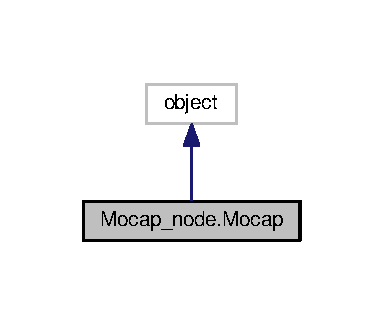
\includegraphics[width=184pt]{classMocap__node_1_1Mocap__inherit__graph}
\end{center}
\end{figure}


Collaboration diagram for Mocap\+\_\+node.\+Mocap\+:
\nopagebreak
\begin{figure}[H]
\begin{center}
\leavevmode
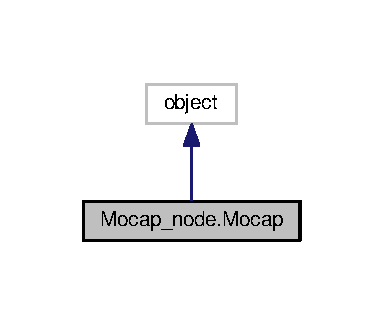
\includegraphics[width=184pt]{classMocap__node_1_1Mocap__coll__graph}
\end{center}
\end{figure}
\subsection*{Public Member Functions}
\begin{DoxyCompactItemize}
\item 
def {\bfseries init} (self)\hypertarget{classMocap__node_1_1Mocap_a105ea248aaefbc083843f694a5e307de}{}\label{classMocap__node_1_1Mocap_a105ea248aaefbc083843f694a5e307de}

\end{DoxyCompactItemize}
\subsection*{Public Attributes}
\begin{DoxyCompactItemize}
\item 
{\bfseries data3}\hypertarget{classMocap__node_1_1Mocap_a77a5eae231614fb9287c311ba6240184}{}\label{classMocap__node_1_1Mocap_a77a5eae231614fb9287c311ba6240184}

\item 
{\bfseries flag}\hypertarget{classMocap__node_1_1Mocap_ad43768099eeb9d60be96078d0cd92cbf}{}\label{classMocap__node_1_1Mocap_ad43768099eeb9d60be96078d0cd92cbf}

\item 
\hyperlink{classMocap__node_1_1Mocap_ab12db5ec1a825bf042d8ad2e82e80116}{flagstart}\hypertarget{classMocap__node_1_1Mocap_ab12db5ec1a825bf042d8ad2e82e80116}{}\label{classMocap__node_1_1Mocap_ab12db5ec1a825bf042d8ad2e82e80116}

\begin{DoxyCompactList}\small\item\em Flag to active the publisher on topic for record. \end{DoxyCompactList}\item 
{\bfseries update\+\_\+rate1}\hypertarget{classMocap__node_1_1Mocap_a58f3c6bbac40bb808d8b4749fcbb0f05}{}\label{classMocap__node_1_1Mocap_a58f3c6bbac40bb808d8b4749fcbb0f05}

\item 
\hyperlink{classMocap__node_1_1Mocap_ac2f9f0ba96350cb83904e470e52a4c61}{data4}\hypertarget{classMocap__node_1_1Mocap_ac2f9f0ba96350cb83904e470e52a4c61}{}\label{classMocap__node_1_1Mocap_ac2f9f0ba96350cb83904e470e52a4c61}

\begin{DoxyCompactList}\small\item\em Frequency (Hz), depends on the used \hyperlink{classMocap__node_1_1Mocap}{Mocap}. \end{DoxyCompactList}\item 
\hyperlink{classMocap__node_1_1Mocap_a4023cc02b52de1a4da63578b5d567990}{pub3}\hypertarget{classMocap__node_1_1Mocap_a4023cc02b52de1a4da63578b5d567990}{}\label{classMocap__node_1_1Mocap_a4023cc02b52de1a4da63578b5d567990}

\begin{DoxyCompactList}\small\item\em publish on a topic the interested data (\textquotesingle{}/mocap\+\_\+data\textquotesingle{}) \end{DoxyCompactList}\end{DoxyCompactItemize}


\subsection{Detailed Description}
class \hyperlink{classMocap__node_1_1Mocap}{Mocap} 

The documentation for this class was generated from the following file\+:\begin{DoxyCompactItemize}
\item 
Mocap\+\_\+node.\+py\end{DoxyCompactItemize}

\hypertarget{classRecorder__IMU_1_1RecorderImu}{}\section{Recorder\+\_\+\+I\+M\+U.\+Recorder\+Imu Class Reference}
\label{classRecorder__IMU_1_1RecorderImu}\index{Recorder\+\_\+\+I\+M\+U.\+Recorder\+Imu@{Recorder\+\_\+\+I\+M\+U.\+Recorder\+Imu}}


class \hyperlink{classRecorder__IMU_1_1RecorderImu}{Recorder\+Imu}  




Inheritance diagram for Recorder\+\_\+\+I\+M\+U.\+Recorder\+Imu\+:
\nopagebreak
\begin{figure}[H]
\begin{center}
\leavevmode
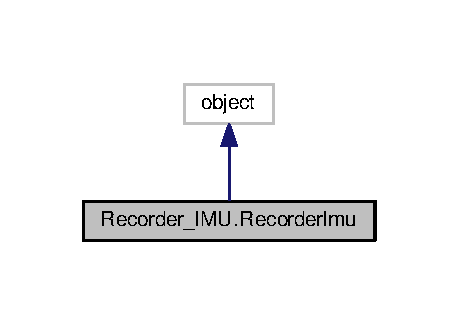
\includegraphics[width=220pt]{classRecorder__IMU_1_1RecorderImu__inherit__graph}
\end{center}
\end{figure}


Collaboration diagram for Recorder\+\_\+\+I\+M\+U.\+Recorder\+Imu\+:
\nopagebreak
\begin{figure}[H]
\begin{center}
\leavevmode
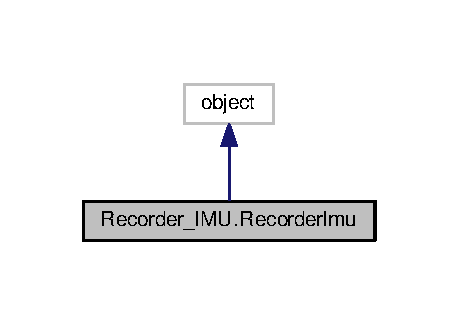
\includegraphics[width=220pt]{classRecorder__IMU_1_1RecorderImu__coll__graph}
\end{center}
\end{figure}
\subsection*{Public Member Functions}
\begin{DoxyCompactItemize}
\item 
def {\bfseries init} (self)\hypertarget{classRecorder__IMU_1_1RecorderImu_adec0cb42c96808ab230f12f43d501340}{}\label{classRecorder__IMU_1_1RecorderImu_adec0cb42c96808ab230f12f43d501340}

\item 
def \hyperlink{classRecorder__IMU_1_1RecorderImu_af8e247022237f2712529d30f1669f996}{callback} (self, data)\hypertarget{classRecorder__IMU_1_1RecorderImu_af8e247022237f2712529d30f1669f996}{}\label{classRecorder__IMU_1_1RecorderImu_af8e247022237f2712529d30f1669f996}

\begin{DoxyCompactList}\small\item\em function for callback \end{DoxyCompactList}\item 
def {\bfseries run} (self)\hypertarget{classRecorder__IMU_1_1RecorderImu_a0a12c640019bac34c7ba3511d91e81de}{}\label{classRecorder__IMU_1_1RecorderImu_a0a12c640019bac34c7ba3511d91e81de}

\end{DoxyCompactItemize}
\subsection*{Public Attributes}
\begin{DoxyCompactItemize}
\item 
\hyperlink{classRecorder__IMU_1_1RecorderImu_a8ebaad8c52eec46a0c8e4c97505f4c93}{working\+Directory}\hypertarget{classRecorder__IMU_1_1RecorderImu_a8ebaad8c52eec46a0c8e4c97505f4c93}{}\label{classRecorder__IMU_1_1RecorderImu_a8ebaad8c52eec46a0c8e4c97505f4c93}

\begin{DoxyCompactList}\small\item\em defining folder \end{DoxyCompactList}\item 
{\bfseries parent\+Directory}\hypertarget{classRecorder__IMU_1_1RecorderImu_a8ea012672caa6aa1cc1735e74bce8075}{}\label{classRecorder__IMU_1_1RecorderImu_a8ea012672caa6aa1cc1735e74bce8075}

\item 
{\bfseries files\+Directory}\hypertarget{classRecorder__IMU_1_1RecorderImu_ad762949b2f90e5e1e3acbbc2223c6a0c}{}\label{classRecorder__IMU_1_1RecorderImu_ad762949b2f90e5e1e3acbbc2223c6a0c}

\item 
{\bfseries data}\hypertarget{classRecorder__IMU_1_1RecorderImu_ada56f1b341c52a87045f6a577967aa5d}{}\label{classRecorder__IMU_1_1RecorderImu_ada56f1b341c52a87045f6a577967aa5d}

\item 
\hyperlink{classRecorder__IMU_1_1RecorderImu_a40c4018904a7166e3bce05b6d84877c2}{flag\+\_\+start}
\begin{DoxyCompactList}\small\item\em creation rosbag \end{DoxyCompactList}\item 
\hyperlink{classRecorder__IMU_1_1RecorderImu_ac4cf806cd47a223064dc935460f43f49}{folder\+\_\+path}\hypertarget{classRecorder__IMU_1_1RecorderImu_ac4cf806cd47a223064dc935460f43f49}{}\label{classRecorder__IMU_1_1RecorderImu_ac4cf806cd47a223064dc935460f43f49}

\begin{DoxyCompactList}\small\item\em saving bag into a defined folder \end{DoxyCompactList}\end{DoxyCompactItemize}


\subsection{Detailed Description}
class \hyperlink{classRecorder__IMU_1_1RecorderImu}{Recorder\+Imu} 

\subsection{Member Data Documentation}
\index{Recorder\+\_\+\+I\+M\+U\+::\+Recorder\+Imu@{Recorder\+\_\+\+I\+M\+U\+::\+Recorder\+Imu}!flag\+\_\+start@{flag\+\_\+start}}
\index{flag\+\_\+start@{flag\+\_\+start}!Recorder\+\_\+\+I\+M\+U\+::\+Recorder\+Imu@{Recorder\+\_\+\+I\+M\+U\+::\+Recorder\+Imu}}
\subsubsection[{\texorpdfstring{flag\+\_\+start}{flag_start}}]{\setlength{\rightskip}{0pt plus 5cm}Recorder\+\_\+\+I\+M\+U.\+Recorder\+Imu.\+flag\+\_\+start}\hypertarget{classRecorder__IMU_1_1RecorderImu_a40c4018904a7166e3bce05b6d84877c2}{}\label{classRecorder__IMU_1_1RecorderImu_a40c4018904a7166e3bce05b6d84877c2}


creation rosbag 

writing into a rosbag 

The documentation for this class was generated from the following file\+:\begin{DoxyCompactItemize}
\item 
Recorder\+\_\+\+I\+M\+U.\+py\end{DoxyCompactItemize}

\hypertarget{classRecorder__mocap_1_1RecorderMocap}{}\section{Recorder\+\_\+mocap.\+Recorder\+Mocap Class Reference}
\label{classRecorder__mocap_1_1RecorderMocap}\index{Recorder\+\_\+mocap.\+Recorder\+Mocap@{Recorder\+\_\+mocap.\+Recorder\+Mocap}}


class \hyperlink{classRecorder__mocap_1_1RecorderMocap}{Recorder\+Mocap}  




Inheritance diagram for Recorder\+\_\+mocap.\+Recorder\+Mocap\+:
\nopagebreak
\begin{figure}[H]
\begin{center}
\leavevmode
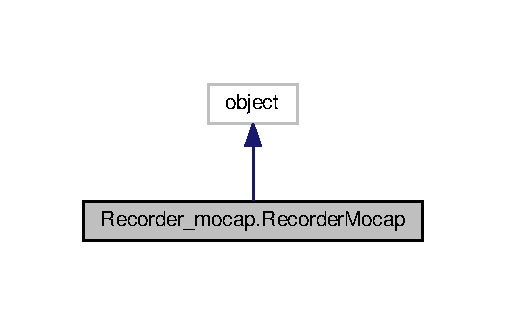
\includegraphics[width=243pt]{classRecorder__mocap_1_1RecorderMocap__inherit__graph}
\end{center}
\end{figure}


Collaboration diagram for Recorder\+\_\+mocap.\+Recorder\+Mocap\+:
\nopagebreak
\begin{figure}[H]
\begin{center}
\leavevmode
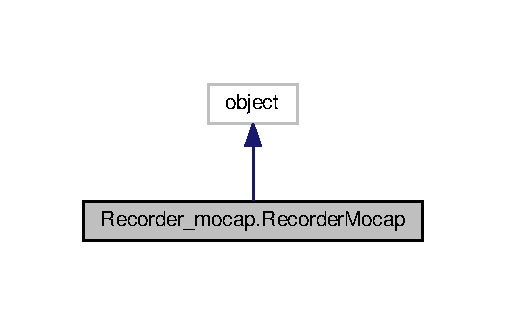
\includegraphics[width=243pt]{classRecorder__mocap_1_1RecorderMocap__coll__graph}
\end{center}
\end{figure}
\subsection*{Public Member Functions}
\begin{DoxyCompactItemize}
\item 
def {\bfseries init} (self)\hypertarget{classRecorder__mocap_1_1RecorderMocap_a9700ab49854d757e0d6c287f0e9f59ef}{}\label{classRecorder__mocap_1_1RecorderMocap_a9700ab49854d757e0d6c287f0e9f59ef}

\end{DoxyCompactItemize}
\subsection*{Public Attributes}
\begin{DoxyCompactItemize}
\item 
{\bfseries working\+Directory}\hypertarget{classRecorder__mocap_1_1RecorderMocap_ad6001fd638bf7e2f6c0340240935883d}{}\label{classRecorder__mocap_1_1RecorderMocap_ad6001fd638bf7e2f6c0340240935883d}

\item 
{\bfseries parent\+Directory}\hypertarget{classRecorder__mocap_1_1RecorderMocap_a63b53ac7be1510948932f3cfdb6a083d}{}\label{classRecorder__mocap_1_1RecorderMocap_a63b53ac7be1510948932f3cfdb6a083d}

\item 
{\bfseries files\+Directory}\hypertarget{classRecorder__mocap_1_1RecorderMocap_aa2e5b4cb986748ed995843370795a089}{}\label{classRecorder__mocap_1_1RecorderMocap_aa2e5b4cb986748ed995843370795a089}

\item 
{\bfseries data}\hypertarget{classRecorder__mocap_1_1RecorderMocap_a57fc29abab5aa54617d975cfffd93368}{}\label{classRecorder__mocap_1_1RecorderMocap_a57fc29abab5aa54617d975cfffd93368}

\item 
\hyperlink{classRecorder__mocap_1_1RecorderMocap_acda19dab01791450a15aa1b4138adf2c}{flag\+\_\+start}\hypertarget{classRecorder__mocap_1_1RecorderMocap_acda19dab01791450a15aa1b4138adf2c}{}\label{classRecorder__mocap_1_1RecorderMocap_acda19dab01791450a15aa1b4138adf2c}

\begin{DoxyCompactList}\small\item\em define the type of message Float32\+Multi\+Array() \end{DoxyCompactList}\end{DoxyCompactItemize}


\subsection{Detailed Description}
class \hyperlink{classRecorder__mocap_1_1RecorderMocap}{Recorder\+Mocap} 

The documentation for this class was generated from the following file\+:\begin{DoxyCompactItemize}
\item 
Recorder\+\_\+mocap.\+py\end{DoxyCompactItemize}

\hypertarget{classRecorder__PC_1_1RecorderPC}{}\section{Recorder\+\_\+\+P\+C.\+Recorder\+PC Class Reference}
\label{classRecorder__PC_1_1RecorderPC}\index{Recorder\+\_\+\+P\+C.\+Recorder\+PC@{Recorder\+\_\+\+P\+C.\+Recorder\+PC}}


class \hyperlink{classRecorder__PC_1_1RecorderPC}{Recorder\+PC}  




Inheritance diagram for Recorder\+\_\+\+P\+C.\+Recorder\+PC\+:
\nopagebreak
\begin{figure}[H]
\begin{center}
\leavevmode
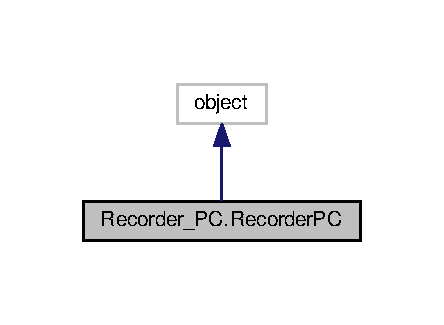
\includegraphics[width=213pt]{classRecorder__PC_1_1RecorderPC__inherit__graph}
\end{center}
\end{figure}


Collaboration diagram for Recorder\+\_\+\+P\+C.\+Recorder\+PC\+:
\nopagebreak
\begin{figure}[H]
\begin{center}
\leavevmode
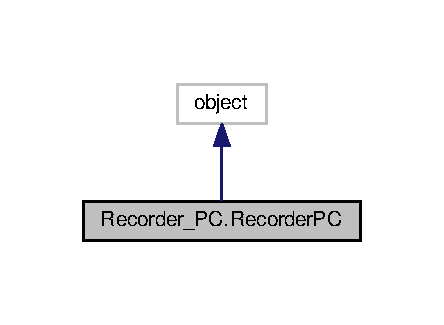
\includegraphics[width=213pt]{classRecorder__PC_1_1RecorderPC__coll__graph}
\end{center}
\end{figure}
\subsection*{Public Member Functions}
\begin{DoxyCompactItemize}
\item 
def {\bfseries init} (self)\hypertarget{classRecorder__PC_1_1RecorderPC_ae8cf41196e47b914112bfd1419d0e7db}{}\label{classRecorder__PC_1_1RecorderPC_ae8cf41196e47b914112bfd1419d0e7db}

\item 
def {\bfseries callback} (self, data)\hypertarget{classRecorder__PC_1_1RecorderPC_a387074d112fd0542749467be5a091ba5}{}\label{classRecorder__PC_1_1RecorderPC_a387074d112fd0542749467be5a091ba5}

\item 
def {\bfseries run} (self)\hypertarget{classRecorder__PC_1_1RecorderPC_af5dcab9276871eb387d633181ec416aa}{}\label{classRecorder__PC_1_1RecorderPC_af5dcab9276871eb387d633181ec416aa}

\end{DoxyCompactItemize}
\subsection*{Public Attributes}
\begin{DoxyCompactItemize}
\item 
\hyperlink{classRecorder__PC_1_1RecorderPC_a2286df16f6de1a1e301abe29040910a1}{working\+Directory}\hypertarget{classRecorder__PC_1_1RecorderPC_a2286df16f6de1a1e301abe29040910a1}{}\label{classRecorder__PC_1_1RecorderPC_a2286df16f6de1a1e301abe29040910a1}

\begin{DoxyCompactList}\small\item\em defining folder \end{DoxyCompactList}\item 
{\bfseries parent\+Directory}\hypertarget{classRecorder__PC_1_1RecorderPC_ae8c8642b704ce3584c15c50ba2cf420e}{}\label{classRecorder__PC_1_1RecorderPC_ae8c8642b704ce3584c15c50ba2cf420e}

\item 
{\bfseries files\+Directory}\hypertarget{classRecorder__PC_1_1RecorderPC_adb58428a92cd66e5cc1a73bb762976d4}{}\label{classRecorder__PC_1_1RecorderPC_adb58428a92cd66e5cc1a73bb762976d4}

\item 
{\bfseries data}\hypertarget{classRecorder__PC_1_1RecorderPC_af4e73c9d38c2e11d0a4fa09be3deebc5}{}\label{classRecorder__PC_1_1RecorderPC_af4e73c9d38c2e11d0a4fa09be3deebc5}

\item 
\hyperlink{classRecorder__PC_1_1RecorderPC_aff33d03c0a4ccab6d6a6b474af57592e}{flag\+\_\+start}
\begin{DoxyCompactList}\small\item\em creation rosbag \end{DoxyCompactList}\item 
\hyperlink{classRecorder__PC_1_1RecorderPC_a4ea59328e25a40d2b28abb963cbaf7f9}{folder\+\_\+path}\hypertarget{classRecorder__PC_1_1RecorderPC_a4ea59328e25a40d2b28abb963cbaf7f9}{}\label{classRecorder__PC_1_1RecorderPC_a4ea59328e25a40d2b28abb963cbaf7f9}

\begin{DoxyCompactList}\small\item\em saving rosbag into a defined folder \end{DoxyCompactList}\end{DoxyCompactItemize}


\subsection{Detailed Description}
class \hyperlink{classRecorder__PC_1_1RecorderPC}{Recorder\+PC} 

\subsection{Member Data Documentation}
\index{Recorder\+\_\+\+P\+C\+::\+Recorder\+PC@{Recorder\+\_\+\+P\+C\+::\+Recorder\+PC}!flag\+\_\+start@{flag\+\_\+start}}
\index{flag\+\_\+start@{flag\+\_\+start}!Recorder\+\_\+\+P\+C\+::\+Recorder\+PC@{Recorder\+\_\+\+P\+C\+::\+Recorder\+PC}}
\subsubsection[{\texorpdfstring{flag\+\_\+start}{flag_start}}]{\setlength{\rightskip}{0pt plus 5cm}Recorder\+\_\+\+P\+C.\+Recorder\+P\+C.\+flag\+\_\+start}\hypertarget{classRecorder__PC_1_1RecorderPC_aff33d03c0a4ccab6d6a6b474af57592e}{}\label{classRecorder__PC_1_1RecorderPC_aff33d03c0a4ccab6d6a6b474af57592e}


creation rosbag 

writing into a rosbag 

The documentation for this class was generated from the following file\+:\begin{DoxyCompactItemize}
\item 
Recorder\+\_\+\+P\+C.\+py\end{DoxyCompactItemize}

%--- End generated contents ---

% Index
\backmatter
\newpage
\phantomsection
\clearemptydoublepage
\addcontentsline{toc}{chapter}{Index}
\printindex

\end{document}
